% Este trabalho está licenciado sob a Licença Atribuição-CompartilhaIgual 4.0 Internacional Creative Commons. Para visualizar uma cópia desta licença, visite http://creativecommons.org/licenses/by-sa/4.0/deed.pt_BR ou mande uma carta para Creative Commons, PO Box 1866, Mountain View, CA 94042, USA.

\chapter{Linguagem de Programação}\label{cap_lingua}

\section{Computador}\label{cap_lim_sec_computador}

\hl{Um computador é um \emph{sistema computacional} de elementos físicos (\emph{hardware}) e elementos lógicos (\emph{software})}.

\hl{O \emph{hardware} são suas partes mecânicas, elétricas e eletrônicas} como: fonte de energia, teclado, mouse/painel tátil, monitor/tela, dispositivos de armazenagem de dados (HDD, \textit{hard disk drive}; SSD, \textit{solid-state drive}; RAM, \textit{random-access memory}; etc.), dispositivos de processamento (CPU, \textit{central processing unit}, GPU, \textit{graphics processing unit}), conectores de dispositivos externos (microfone, caixa de som, fone de ouvido, USB, etc.), placa mãe, etc..

\hl{O \emph{software} é toda a informação processada pelo computador}, qualquer código executado e qualquer dado usado nas computações.

\begin{figure}[H]
  \centering
  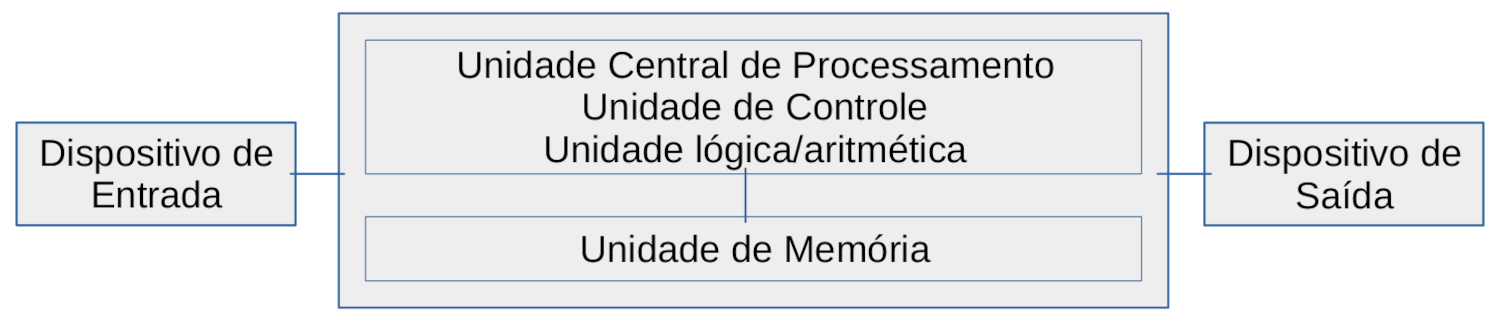
\includegraphics[width=4.75in]{./cap_lingua/dados/fig_arqVonNeumann/fig.png}
  \caption[Arquitetura de von Neumann]{Arquitetura de computador de von Neumann.}
  \label{cap_lim_sec_computador:fig:arqVonNeumann}
\end{figure}

Os computadores que comumente utilizamos seguem a arquitetura de John von Neumann{\vonNeumann}, que consiste em dispositivo(s) de entrada de dados, unidade(s) de processamento, unidade(s) de memória e dispositivo(s) de saída de dados (Figura~\ref{cap_lim_sec_computador:fig:arqVonNeumann}).

\ifisbook
\newpage
\fi

\begin{itemize}
\item \hlemph{Dispositivos de entrada e saída}

  São elementos do computador que permitem a comunicação humana (usuária(o)) com a máquina.

  \begin{itemize}
  \item \hlemph{Dispositivos de entrada}

    São elementos que permitem o fluxo de informação da(o) usuária(o) para a máquina. Exemplos são: teclado, mouse/painel tátil, microfone, etc.

  \item \hlemph{Dispositivos de saída}

    São elementos que permitem o fluxo de informação da máquina para a(o) usuária(o). Exemplos são: monitor/tela, alto-falantes, luzes espia, etc.
  \end{itemize}

\item \hlemph{Unidade central de processamento}

  A \emph{CPU} (do inglês, \textit{Central Processing Unit}) é o elemento que processa as informações e é composta de \emph{unidade de controle}, \emph{unidade lógica e aritmética} e de \emph{memória cache}.

  \begin{itemize}
  \item \hlemph{Unidade de controle}

    Coordena as execuções do processador: busca e decodifica instruções, lê e escreve no \textit{cache} e controla o fluxo de dados.

  \item \hlemph{Unidade lógica/aritmética}

    Executa as instruções operações lógicas e aritméticas, por exemplo: executar a adição, multiplicação, testar se dois objetos são iguais, etc.

  \item \hlemph{Memória cache}

    Memória interna da CPU muito mais rápida que as memórias RAM e dispositivos e armazenamento HDD/SSD. É um dispositivo de memória de pequena capacidade e é utilizada como memória de curto prazo e diretamente acessada.
  \end{itemize}

\item \hlemph{Unidades de memória}

  As unidades de memória são elementos que permitem o armazenamento de dados/objetos. Como memória principal tem-se a \emph{ROM} (do inglês, \textit{Read Only Memory}) e a \emph{RAM} (do inglês, \textit{Random Access Memory}) e como memória de massa/secundária tem-se HDD, SSD, entre outras.

\item \hlemph{Memória ROM}

  A memória ROM é utilizada para armazenamento de dados/objetos necessários para dar início ao funcionamento do computador. Por exemplo, é onde a BIOS (dos inglês, \textit{Basic Input/Output System}, Sistema Básico de Entrada e Saída) é armazenada. Ao ligarmos o computador este programa é iniciado e é responsável por fazer o gerenciamento inicial dos diversos dispositivos do computador e carregar o \emph{sistema operacional} (conjunto de programas cuja função é de gerenciar os recursos do computador e controlar a execução de programas).

\item \hlemph{Memória RAM}

  Memória de acesso rápido utilizada para dados/objetos de uso frequente durante a execução de programas. É uma memória volátil, i.e. toda a informação guardada nela é perdida quando o computador é desligado.

\item \hlemph{Memória de massa/secundária}

  Memória de massa ou secundária são usadas para armazenar dados/objetos por período longo. Normalmente, são dispositivos HDD ou SSD, os dados/objetos são guardados mesmo que o computador seja desligado e contém grande capacidade de armazenagem.   
\end{itemize}

\hl{Os \emph{software} são os elementos lógicos de um sistema computacional, são programas de computadores que contém as instruções que gerenciam o \emph{hardware} para a execução de tarefas específicas}, por exemplo, imprimir um texto, gravar áudio/vídeo, resolver um problema matemático, etc. Programar é o ato de criar programas de computadores.

\subsection{Linguagem de Programação}

\hl{As informações fluem no computador codificadas como registros de \textit{bits}}\footnote{Usualmente, de tamanho $64$-\textit{bits}.}\hl{ (sequência de zeros ou uns)}. Há registros de instrução e de dados. Programar diretamente por registros é uma tarefa muito difícil, o que levou ao surgimento de linguagens de programação. \hl{Uma \emph{linguagem de programação}}\footnote{Código de programação, código de máquina ou linguagem de máquina.}\hl{ é um método padronizado para escrever instruções para execução de tarefas no computador}. As instruções escritas em uma linguagem são interpretadas e/ou compiladas por um software (interpretador ou compilador) da linguagem que decodifica as instruções em registros de instruções e dados, os quais são efetivamente executados na máquina.

Existem várias linguagens de programação disponíveis e elas são classificadas por diferentes características. Uma \emph{linguagem de baixo nível} (por exemplo, \href{https://pt.wikipedia.org/wiki/Linguagem_assembly}{Assembly}) é aquela que se restringe às instruções executadas diretamente pelo processador, enquanto que uma \emph{linguagem de alto nível} contém instruções mais complexas e abstratas. Estas contém sintaxe mais próxima da linguagem humana natural e permitem a manipulação de objetos mais abstratos. Exemplos de linguagens de alto nível são: \href{https://pt.wikipedia.org/wiki/BASIC}{Basic}, \href{https://pt.wikipedia.org/wiki/Java\_(linguagem\_de\_programa\%C3\%A7\%C3\%A3o)}{Java}, \href{https://pt.wikipedia.org/wiki/JavaScript}{Javascript}, \href{https://pt.wikipedia.org/wiki/MATLAB}{MATLAB}, \href{https://pt.wikipedia.org/wiki/PHP}{PHP}, \href{https://pt.wikipedia.org/wiki/R\_(linguagem_de_programa\%C3\%A7\%C3\%A3o)}{R}, \href{https://pt.wikipedia.org/wiki/C\%2B\%2B}{C/C++}, {\python}, etc.

\hl{Em geral, não existe uma melhor linguagem, cada uma tem suas características que podem ser mais ou menos adequadas conforme o programa que se deseja desenvolver}. Por exemplo, para um site de internet, linguagens como \href{https://pt.wikipedia.org/wiki/JavaScript}{Javascript} e \href{https://pt.wikipedia.org/wiki/PHP}{PHP} são bastante úteis, mas não no desenvolvimento de modelagem matemática e computacional. Nestes casos, \href{https://pt.wikipedia.org/wiki/C\%2B\%2B}{C/C++} é uma linguagem mais apropriada por conter várias estruturas de programação que facilitam a modelagem computacional de problemas científicos. Agora, \href{https://pt.wikipedia.org/wiki/R\_(linguagem_de_programa\%C3\%A7\%C3\%A3o)}{R} é uma linguagem de alto nível com diversos recursos dedicados às áreas de ciências de dados e estatística. Usualmente, utiliza-se mais de uma linguagem no desenvolvimento de programas mais avançados. A ideia é de explorar o melhor de cada linguagem na criação de programas eficientes na resolução dos problemas de interesse.

Nestas notas de aula, \hl{{\python}} é a linguagem escolhida para estudarmos algoritmos e programação. Trata-se de uma \hl{linguagem de alto nível, \emph{interpretada}, \emph{dinâmica} e \emph{mutiparadigma}}. Foi lançada por Guido van Rossum{\rossum} em 1991 e, atualmente, é desenvolvida de forma comunitária, aberta e gerenciada pela ONG \href{https://pt.wikipedia.org/wiki/Python_Software_Foundation}{Python Software Foundation}. A linguagem foi projetada para priorizar a legibilidade do código. Parte da filosofia da linguagem é descrita pelo poema \href{https://pt.wikipedia.org/wiki/Zen_de_Python}{The Zen of Python}. Pode-se lê-lo pelo \textit{easter egg} {\python}:

\begin{lstlisting}
>>> import this
\end{lstlisting}

\begin{itemize}
\item \hlemph{Linguagem interpretada}

  {\python} é uma linguagem interpretada. Isso significa que o \emph{código-fonte} escrito em linguagem {\python} é interpretado por um programa (interpretador {\python}). Ao executar-se um código, o interpretador lê uma linha do código, decodifica-a como registros para o processador que os executa. Executada uma linha, o interpretador segue para a próxima até o código ter sido completadamente executado.

\item \hlemph{Linguagem compilada}

  Em uma linguagem compilada, como \href{https://pt.wikipedia.org/wiki/C\%2B\%2B}{C/C++}, há um programa chamado de \emph{compilador} (em inglês, \textit{compiler}) e outro de \emph{ligador} (em inglês, \textit{linker}). O primeiro, cria um programa-objeto a partir do código e o segundo gerencia sua ligação com eventuais bibliotecas computacionais que ele possa depender. O programa-objeto (também chamado de executável) pode então ser executado pela máquina.
\end{itemize}

Em geral, a execução de um programa compilado é mais rápida que a de um código interpretado. De forma simples, isso se deve ao fato de que nesse a interpretação é feita toda de uma vez e não precisa ser refeita na execução de cada linha de código, como no segundo caso. Por outro lado, a compilação de códigos-fonte grandes pode ser bastante demorada fazendo mais sentido quando ele é compilado uma vez e o programa-objeto executado várias vezes. Além disso, linguagens interpretadas podem usar bibliotecas de programas pré-compiladas. Com isso, pode-se alcançar um bom balanceamento entre tempo de desenvolvimento e de execução do código.

O interpretador {\python} também pode ser usado para compilar o código para um arquivo \emph{bytecode}, este é executado muito mais rápido do que o código-fonte em si, pois as interpretações necessárias já foram feitas. Mais adiante, vamos estudar isso de forma mais detalhada.

\ifisbook
\newpage
\fi

\begin{itemize}
\item \hlemph{Linguagem de tipagem dinâmica}

  {\python} é uma linguagem de tipagem dinâmica. Nela, os dados não precisam ser explicitamente tipificados no código-fonte e o interpretador os tipifica com base em regras da própria linguagem. Ao executar operações com os dados, o interpretador pode alterar seus tipos de forma dinâmica.

\item \hlemph{Linguagem de tipagem estática}

  \href{https://pt.wikipedia.org/wiki/C\%2B\%2B}{C/C++} é um exemplo de uma linguagem de tipagem estática. Em tais linguagens, os dados devem ser explicitamente tipificados no código-fonte com base nos tipos disponíveis. A retipificação pode ocorrer, mas precisa estar explicitamente definida no código.
\end{itemize}

Existem vários \emph{paradigmas de programação} e a \hl{linguagem {\python} é multiparadigma}, i.e. permite a utilização de mais de um no código-fonte. Exemplos de paradigmas de programação são: \emph{estruturada}, \emph{orientada a objetos}, \emph{orientada a eventos}, etc.. Na maior parte destas notas de aulas, vamos estudar algoritmos para linguagens de programação estruturada. Mais ao final, vamos introduzir aspectos de linguagens orientada a objetos. Estes são paradigmas de programação fundamentais e suas estruturas são importantes na programação com demais paradigmas disponíveis em programação de computadores.

\subsection{Instalação e Execução}

\hl{{\python} é um \emph{software aberto}}\footnote{Consulte a licença de uso em \url{https://docs.python.org/3/license.html}.} e está disponível para vários sistemas operacionais ({\linux}, macOS, Windows, etc.) no seu site oficial
\begin{center}
  \url{https://www.python.org/}
\end{center}
Também, está disponível (gratuitamente) na loja de aplicativos dos sistemas operacionais mais usados. Esta costuma ser a forma mais fácil de instalá-lo na sua máquina, consulte a loja de seus sistema operacional. Ainda, há plataformas e IDEs\footnote{IDE, do inglês, \textit{integrated development enviroment}, ambiente de desenvolvimento integrado} {\python} disponíveis, consulte, como por exemplo, \href{https://www.anaconda.com/}{Anaconda}.

A execução de um código {\python} pode ser feita de várias formas.

\begin{itemize}
\item \hlemph{Execução iterativa via terminal}

  Em terminal {\python} pode-se executar instruções/comandos de forma iterativa. Por exemplo:

\begin{lstlisting}[xrightmargin=2.5em]
>>> print('Olá, mundo!')
Olá, mundo!
>>> 
\end{lstlisting}      

  \hl{O símbolo }\lstinline+>>>+\hl{ denota o \emph{prompt de entrada}, onde uma instrução {\python} pode ser digitada}. Após digitar, o comando é executada teclando \lstinline+<ENTER>+. Caso o comando tenha alguma \hl{saída de dados}, como no caso acima, esta aparecerá, por padrão, \hl{no \emph{prompt de saída}}, logo abaixo a linha de comando executada. \hl{Um novo símbolo de prompt de entrada aparece ao término da execução anterior}.

\item \hlemph{Execução de um \textit{script}}

  Para códigos com várias linhas de instruções é mais adequado utilizar um aquivo de \textit{script} {\python}. Usando-se um editor de texto ou um IDE ditam-se as linhas de comando em um arquivo \lstinline+.py+. Então, \textit{script} pode ser executado em um terminal de seu sistema operacional utilizando-se o interpretador {\python}. Por exemplo, assumindo que o código for salvo do arquivo \lstinline+path_to_arq/arq.py+, pode-se executá-lo em um terminal do sistema com

\begin{lstlisting}[xrightmargin=2.5em]
$ python3 path_to_arq/arq.py 
\end{lstlisting}%$
  

  IDEs para {\python} fornecem uma ambiente integrado, contendo um campo para escrita do código e terminal {\python} integrado. Consulte, por exemplo, o IDE {\spyder}:
  \begin{center}
    \url{https://www.spyder-ide.org/}
  \end{center}

\item \hlemph{Execução em um \textit{notebook}}

  \textit{Notebooks} {\python} são uma boa alternativa para a execução de códigos em um ambiente colaborativo/educativo. Por exemplo, {\jupyter} é um notebook que roda em navegadores de internet. Sua estrutura e soluções também são encontradas em notebooks online (de uso gratuito limitado) como {\colab} e {\kaggle}.  
\end{itemize}

\subsection{Exercícios}

% exercícios de compreensão

\begin{exer}
  Complete as lacunas.
  \begin{enumerate}[a)]
    \item \underline{\phantom{\textit{Hardware}}} é um elemento físico de um computador.
    \item \textit{Software} é um elemento \underline{\phantom{lógico}} de um computador.
    \item Teclado e \textit{mouse} são exemplos de dispositivos de \underline{\phantom{entrada}} de dados em um computador.
    \item Monitor/tela e auto-falantes são exemplos de \underline{\phantom{dispositivos de saída}} de dados em um computador.
    \item \underline{\phantom{CPU}} é um dos elementos que processa as informações em um computador.
    \item As \underline{\phantom{unidades de memória}} são elementos que permitem o armazenamento de dados/objetos.
  \end{enumerate}
\end{exer}
\begin{resp}
  a) \textit{Hardware}; b) lógico; c) entrada; d) dispositivos de saída; e) CPU; f) unidades de memória.
\end{resp}

\begin{exer}
  Complete as lacunas.
  \begin{enumerate}[a)]
    \item Uma linguagem de programação é um método para escrever instruções para a execução de \underline{\phantom{tarefas}} no computador.
    \item {\python} é uma linguagem de \underline{\phantom{alto}} nível, de tipagem \underline{\phantom{dinâmica}} e multiparadigma.
  \end{enumerate}
\end{exer}
\begin{resp}
  a) tarefas; b) alto; dinâmica
\end{resp}

% exercícios

\begin{exer}
  Verifique qual a versão do sistema operacional que está utilizado em seu computador.
\end{exer}
\begin{resp}
  Dica: no seu sistema operacional, busque pelas informações do sistema.
\end{resp}

\begin{exer}
  Verifique os seguintes elementos de seu computador:
  \begin{enumerate}[a)]
  \item CPUs
  \item Placa(s) gráfica(s)
  \item Memória RAM
  \item Armazenamento HDD/SSD.
  \end{enumerate}
\end{exer}
\begin{resp}
  Dica: no seu sistema, busque pelas informações do sistema.
\end{resp}

\begin{exer}
  Verifique como entrar na \lstinline+BIOS+ de seu computador. Atenção! Não faça e salve nenhuma alteração. Modificações na \lstinline+BIOS+ podem impedir que seu computador funcione normalmente, inclusive, impedir que você inicialize seu sistema operacional.
\end{exer}
\begin{resp}
  Dica: cada computador tem sua forma de acessar a \lstinline+BIOS+. Verifique o manual ou busque na \textit{web} pela marca e modelo de seu computador.
\end{resp}

\begin{exer}
  Instale {\python} no seu computador (caso ainda não tenha feito) e abra um terminal {\python}. Nele, escreva uma linha de comando que imprima no prompt de saída a frase ``Olá, meu Python!''.
\end{exer}
\begin{resp}

\begin{lstlisting}
>>> print('Olá, meu Python!')
Olá, meu Python!
>>> 
\end{lstlisting}

\end{resp}

\begin{exer}
  Instale um IDE para {\python} no seu computador (caso ainda não tenha feito) e use-o para escrever o seguinte \textit{script}

\begin{lstlisting}
import math as m
print(f'Número pi = {m.pi}')
print(f'Número de Euler e = {m.e}')
\end{lstlisting}

  Também, execute o \textit{script} diretamente em um terminal de seu sistema operacional.
\end{exer}
\begin{resp}
  Dica: instale o IDE {\spyder}, disponível em
  \begin{center}
    \url{https://www.spyder-ide.org/}
  \end{center}
\end{resp}

\begin{exer}
  Use um \textit{notebook} {\python} para escrever e executar o código do exercício anterior.
\end{exer}
\begin{resp}
  Dica: use um notebook online {\colab} (\url{https://colab.research.google.com/}), {\kaggle} (\url{https://www.kaggle.com/}) ou {\jupyter} (\url{https://jupyter.org/}).
\end{resp}

\ifisbook
\subsubsection{Respostas}
\shipoutAnswer
\fi

\section{Algoritmos e Programação}\label{cap_lingua_sec_algoprog}

\hl{\emph{Programar} é criar um programa} (um \textit{software}) \hl{para ser executado em computador}. Para isso, escreve-se \hl{um código em uma linguagem computacional} (por exemplo, em {\python}), o qual é interpretado/compilado para gerar o programa final. \hl{Linguagens computacionais são técnicas, utilizam uma sintaxe simples, precisa e sem ambiguidades}. Ou seja, para criarmos um programa com um determinado objetivo, precisamos escrever um código computacional técnico, que siga a sintaxe da linguagem escolhida e sem ambiguidades.

\hl{Um \emph{algoritmo} pode ser definido uma sequencia ordenada e sem ambiguidade de passos para a resolução de um problema}.

\begin{ex}\label{cap_lingua_sec_algoprog:ex:areaTriang}
O cálculo da área de um triângulo de base e altura dadas por ser feito com o seguinte algoritmo:
\begin{enumerate}
\item Informe o valor da base $b$.
\item Informe o valor da altura $h$.
\item $\displaystyle a \leftarrow \frac{b\cdot h}{2}$.
\item Imprima o valor de $a$.
\end{enumerate}

\hl{Algoritmos para a programação são pensados para serem facilmente transformados em códigos computacionais}. Por exemplo, o algoritmo acima pode ser escrito em {\python} como segue:

\begin{lstlisting}
b = float(input('Informe o valor da base.\n'))
h = float(input('Informe o valor da altura.\n'))
# cálculo da área
a = b*h/2
print(f'Área = {a}')
\end{lstlisting}

\end{ex}

Para criar um programa para resolver um dado problema, começamos desenvolvendo um algoritmo para resolvê-lo, este algoritmo é implementado na linguagem computacional escolhida, a qual gera o programa final. Aqui, o passo mais difícil costuma ser o desenvolvimento do algoritmo. Precisamos pensar em como podemos resolver o problema de interesse em uma sequência de passos ordenada e sem ambiguidades para que possamos implementá-los em computador.

\hl{Um algoritmo deve ter as seguintes propriedades}:
\begin{itemize}
\item \hl{Cada passo deve estar bem definido}, i.e. não pode conter ambiguidades.
\item \hl{Cada passo deve contribuir de forma efetiva na solução do problema}.
\item \hl{Deve ter número finito de passos} que podem ser \hl{computados em um tempo finito}.
\end{itemize}

\begin{obs}\normalfont{(\hl{Mulher na Matemática}.)}
  A primeira pessoa a publicar um algoritmo para programação foi \hl{Augusta Ada King}{\lovelace}. O algoritmo foi criado para computar os \href{https://pt.wikipedia.org/wiki/N\%C3\%BAmeros\_de\_Bernoulli}{números de Bernoulli}{\bernoulli}.
\end{obs}


\subsection{Fluxograma}

\hl{Fluxograma é uma representação gráfica de um algoritmo}. Entre outras, usam-se as seguintes formas para representar tipos de ações a serem executadas:

\begin{itemize}
\item \hlemph{Terminal}: início ou final do algoritmo.
  \begin{center}
    
\includegraphics[width=0.75in]{./cap_lingua/dados/fig_fluxograma/terminal.png}
  \end{center}  
\item \hlemph{Linha de fluxo}: direciona para a próxima execução.
  \begin{center}
    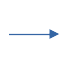
\includegraphics[width=0.75in]{./cap_lingua/dados/fig_fluxograma/linha.png}
  \end{center}
\item \hlemph{Entrada}: leitura de informação/dados.
  \begin{center}
    
\includegraphics[width=0.75in]{./cap_lingua/dados/fig_fluxograma/entrada.png}
  \end{center}  
\item \hlemph{Processo}: ação a ser executada.
  \begin{center}
    
\includegraphics[width=0.75in]{./cap_lingua/dados/fig_fluxograma/processo.png}
  \end{center}
\item \hlemph{Decisão}: ramificação do processamento baseada em uma condição.
  \begin{center}
    
\includegraphics[width=0.75in]{./cap_lingua/dados/fig_fluxograma/decisao.png}
  \end{center}
\item \hlemph{Saída}: impressão de informação/dados.
  \begin{center}
    
\includegraphics[width=0.75in]{./cap_lingua/dados/fig_fluxograma/saida.png}
\end{center}
\end{itemize}

\begin{ex}\label{cap_lingua_sec_algoprog:ex:metHeron}
  O \href{https://en.wikipedia.org/wiki/Methods_of_computing_square_roots#Heron's_method}{método de Heron}{\heron} é um algoritmo para o cálculo aproximado da raiz quadrada de um dado número $x$, i.e. $\sqrt{x}$. Consiste na iteração
  \begin{align}
    s^{(0)} &= \text{approx. inicial},\\
    s^{(i+1)} &= \frac{1}{2}\left(s^{(i)} + \frac{x}{s^{(i)}}\right),
  \end{align}
  para $i=0,1,2,\ldots,n$, onde $n$ é o número de iterações calculadas.

  Na sequência, temos um algoritmo e seus fluxograma e código {\python} para computar a quarta aproximação de $\sqrt{x}$, assumindo $s^{(0)} = x/2$ como aproximação inicial.

  \begin{figure}[ht]
    \centering
    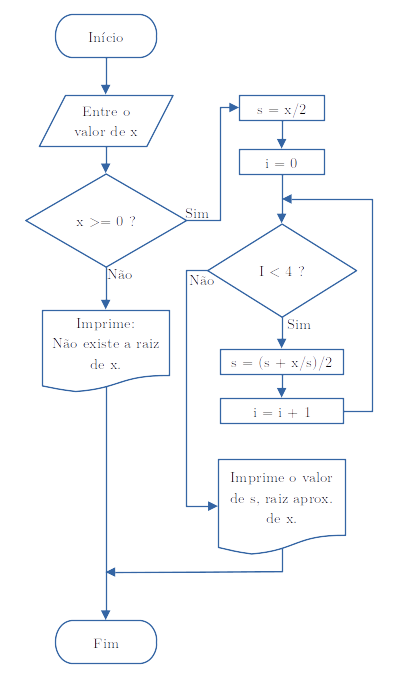
\includegraphics[height=5in]{./cap_lingua/dados/fig_fluxograma/fig.png}
    \caption{Fluxograma referente ao Exemplo~\ref{cap_lingua_sec_algoprog:ex:metHeron}.}
    \label{cap_lingua_sec_algoprog:fig:metHeron}
  \end{figure}

  \begin{itemize}
  \item \emph{Algoritmo}
    \begin{enumerate}
    \item Entre o valor de $x$.
    \item Se $x\geq 0$, faça:
      \begin{enumerate}
      \item $s \leftarrow x/2$
      \item Para $i = 0,1,2,3$, faça:
        \begin{enumerate}
        \item $s \leftarrow (s + x/s)/2$.
        \end{enumerate}
      \item Imprime o valor de $s$.
      \end{enumerate}
    \item Senão, faça:
      \begin{enumerate}
      \item Imprime mensagem ``Não existe!''.
      \end{enumerate}
    \end{enumerate}

  \item \emph{Fluxograma}
  
    Consulte a Figura~\ref{cap_lingua_sec_algoprog:fig:metHeron}.
    
  \item \emph{Código {\python}}

\begin{lstlisting}[caption=metHeron.py,label=cap_lingua_sec_algoprog:cod:metHeron, xrightmargin=2.5em]
x = float(input('Entre com o valor de x: '))
if (x >= 0.):
    s = x/2
    for i in range(4):
        s = (s + x/s)/2
    print(f'Raiz aprox. de x = {s}')
else:
    print(f'Não existe!')
\end{lstlisting}

  \end{itemize}

  O algoritmo tem um \textit{bug} (um erro)! Consulte o Exercício~\ref{cap_lingua_sec_algoprog:exer:bugHeron}.
\end{ex}

\hl{Algoritmos escritos em uma forma próxima de uma linguagem computacional} são, também, chamados de \hl{\emph{pseudocódigos}}. Na prática, pseudocódigos e fluxogramas são usados para apresentar uma forma mais geral e menos detalhada de um algoritmo. Usualmente, sua forma detalhada é escrita diretamente em uma linguagem computacional escolhida.

\subsection{Exercícios}

\begin{exer}
  Complete as lacunas.
  \begin{enumerate}[a)]
    \item Programar é desenvolver um \underline{\phantom{\textit{software}}} para ser executado em um computador.
    \item Linguagens computacionais tem uma \underline{\phantom{sintaxe}} simples, precisa e sem ambiguidades.
    \item Um algoritmo é uma sequência finita de passos \underline{\phantom{bem definidos}} que permitem a resolução \underline{\phantom{objetiva}} de um problema em tempo \underline{\phantom{finito}}.
    \item \underline{\phantom{Pseudocódigo}} é um algoritmo escrito em uma forma próxima de uma linguagem computacional.
  \end{enumerate}
\end{exer}
\begin{resp}
  a) programa/código/\textit{software}. b) sintaxe. c) bem definidos; objetiva; finito. d) Pseudocódigo.
\end{resp}

\begin{exer}
  Complete as lacunas.
  \begin{enumerate}[a)]
    % a)
    \item \underline{\phantom{Fluxograma}} é uma representação gráfica de um algoritmo.
    % b)
    \item Em um fluxograma, \underline{\phantom{terminal}} indicada o início ou final de um algoritmo.
    % c)
    \item A \underline{\phantom{linha de fluxo}} direciona para o próximo bloco de \underline{\phantom{execução}}.
    % d)
    \item A leitura de dados é indicada por um bloco de \underline{\phantom{entrada}} em um fluxograma.
    % e)
    \item Um bloco de \underline{\phantom{processo}} indica uma ação a ser executada.
    % f)
    \item Uma ramificação do algoritmo é indicada no seu fluxograma por um bloco de \underline{\phantom{decisão}}.
    % g
    \item Em um fluxograma, o bloco de \underline{\phantom{saída}} indica a impressão de um dado.
  \end{enumerate} 
\end{exer}
\begin{resp}
  a) Fluxograma. b) terminal. c) linha de fluxo; execução. d) entrada. e) processo. f) decisão. g) saída.
\end{resp}

\begin{exer}
  Escreva um algoritmo/pseudocódigo e um fluxograma correspondente computar a média aritmética entre dois números $x$ e $y$ dados. Como desafio, tente escrever um código {\python} baseado em seu algoritmo.
\end{exer}
\begin{resp}
  \begin{itemize}
    \item Algoritmo
    
\begin{verbatim}
1. Entre com os valores de x e y
2. m = (x + y)/2
3. Imprime m
\end{verbatim}

    \item Fluxograma

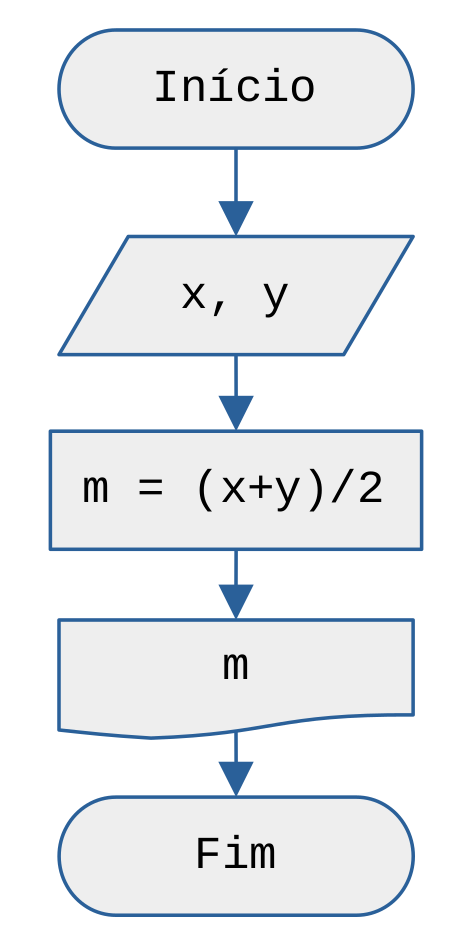
\includegraphics[width=1in]{./cap_lingua/dados/fig_resp_media/fig.png}

  \end{itemize}
\end{resp}

\begin{exer}
  Escreva um algoritmo/pseudocódigo e um fluxograma correspondente para computar a área de um quadrado de lado $l$ dado. Como desafio, tente escrever um código {\python} baseado em seu algoritmo.
\end{exer}
\begin{resp}
  \begin{itemize}
    \item Algoritmo

\begin{verbatim}
1. Entre com o valor de l
2. area = l*l
3. Imprime area
\end{verbatim}

  \end{itemize}
\end{resp}

\begin{exer}
  Escreva um algoritmo/pseudocódigo e um fluxograma correspondente para computar a área de um retângulo de lados $a, b$ dados. Como desafio, tente escrever um código {\python} baseado em seu algoritmo.
\end{exer}
\begin{resp}

\begin{verbatim}
1. Entre com o valor de a
2. Entre com o valor de b
3. area = a*b
4. Imprime area
\end{verbatim}

\end{resp}


\begin{exer}
  Escreva um algoritmo/pseudocódigo e um fluxograma correspondente para computar a área de um triângulo retângulo de dada hipotenusa $h$ e um dos lados $l$ dado. Como desafio, tente escrever um código {\python} baseado em seu algoritmo.
\end{exer}
\begin{resp}
  \begin{itemize}
    \item Algoritmo

\begin{verbatim}
1. Entre com o valor de h
2. Entre com o valor de l
#  o outro cateto
3. m = sqrt(h*h - l*l)
4. area = m*l/2.
5. Imprime area
\end{verbatim}

\item Fluxograma

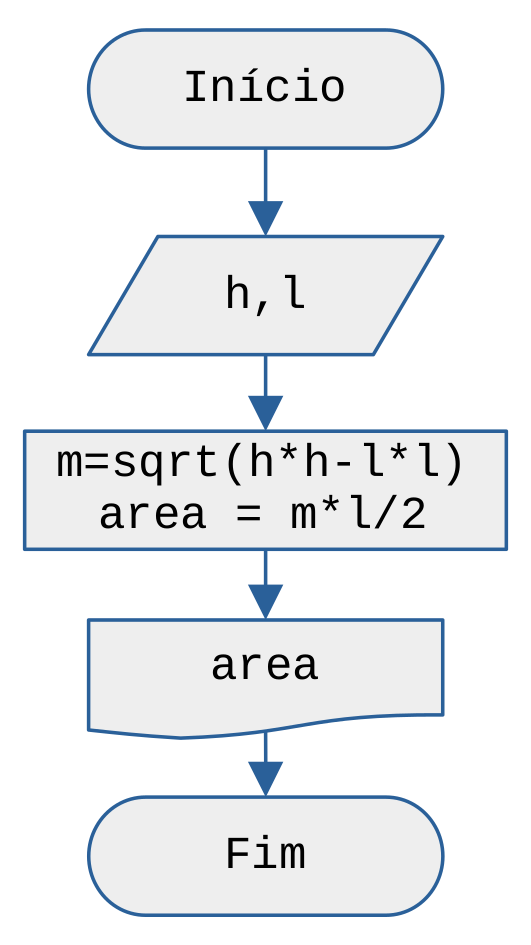
\includegraphics[width=1.15in]{./cap_lingua/dados/fig_resp_triaRet/fig.png}

  \end{itemize}
\end{resp}

\begin{exer}
  Escreva um algoritmo/pseudocódigo e um fluxograma correspondente para computar o zero de uma função afim
  \begin{equation}
    f(x) = ax + b,
  \end{equation}
  dados os coeficientes $a$ e $b$. Como desafio, tente escrever um código {\python} baseado em seu algoritmo.
\end{exer}
\begin{resp}

\begin{verbatim}
1. Entre com o valor de a
2. Entre com o valor de b
3. x0 = -b/a
4. Imprime x0
\end{verbatim}
  
\end{resp}  

\begin{exer}
  Escreva um algoritmo/pseudocódigo e um fluxograma correspondente para computar as raízes reais de um polinômio quadrático
  \begin{equation}
    p(x) = ax^2 + bx + c,
  \end{equation}
  dados os coeficientes $a$, $b$ e $c$. Como desafio, tente escrever um código {\python} baseado em seu algoritmo.
\end{exer}
\begin{resp}

\begin{verbatim}
1. Entre com o valor de a
2. Entre com o valor de b
3. Entre com o valor de c
#  discriminante
4. delta = b*b - 4.*a*c
#  raízes
5. x1 = (-b - sqrt(delta))/2.
6. x2 = (-b + sqrt(delta))/2.
7. Imprime x1 e x2
\end{verbatim}
  
\end{resp}

\begin{exer}
  A \href{https://pt.wikipedia.org/wiki/S%C3%A9rie_harm%C3%B3nica_(matem%C3%A1tica)}{Série Harmônica} é defina por
  \begin{equation}
    \sum_{k=1}^\infty\frac{1}{k} := \frac{1}{1} + \frac{1}{2} + \frac{1}{3} + \cdots
  \end{equation}
  Escreva um algoritmo/pseudocódigo e um fluxograma corresponde para computar o valor da série harmônica truncada em $k=n$, com $n$ dado. Ou seja, dado $n$, o objetivo é calcular
  \begin{equation}
    \sum_{k=1}^n\frac{1}{k} := \frac{1}{1} + \frac{1}{2} + \cdots + \frac{1}{n}.
  \end{equation}
\end{exer}
\begin{resp}
\begin{itemize}
  \item Algoritmo
  
\begin{verbatim}
1. Entre com o valor de n.
2. s = 0.
3. Para i = 1, 2, ... n:
3.1. s = s + 1./i
4. Imprime s
\end{verbatim}

  \item Fluxograma

  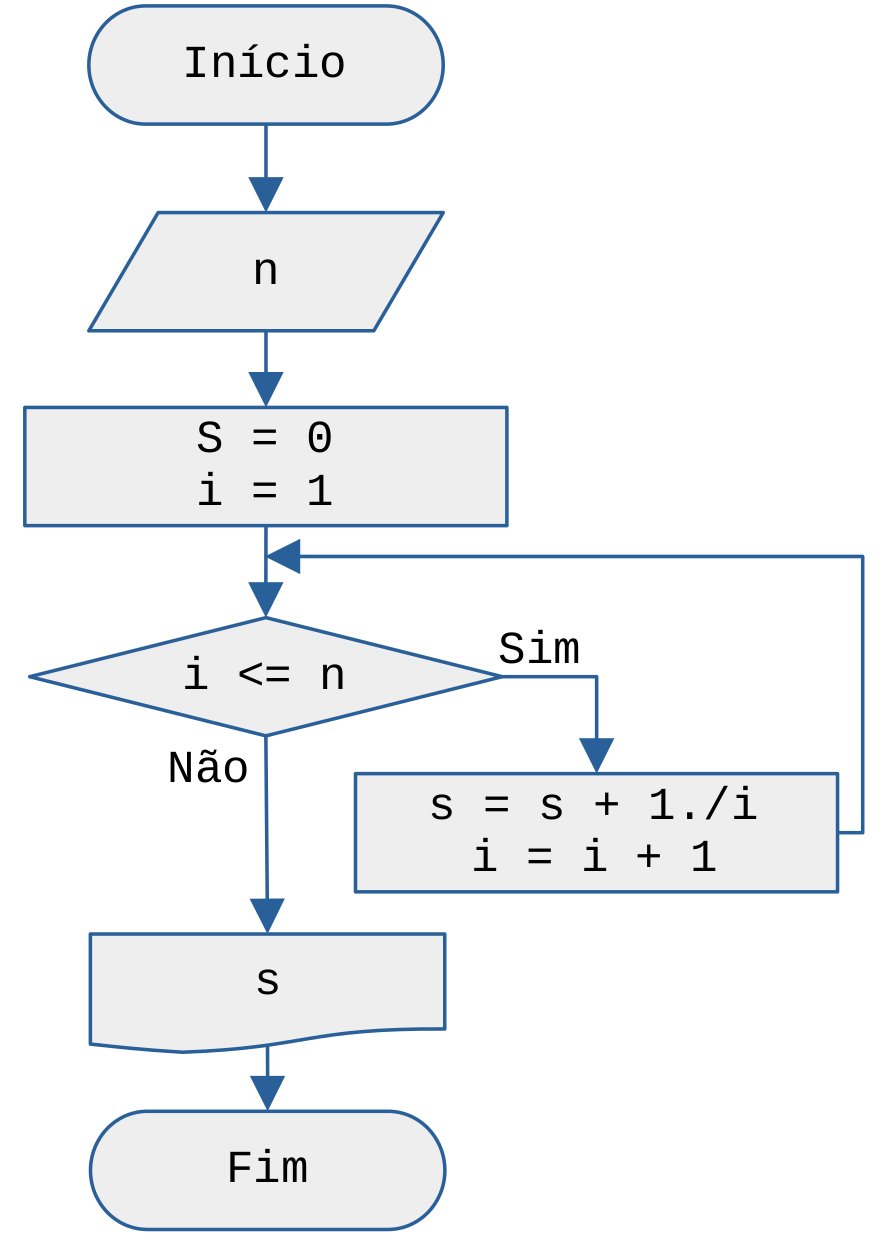
\includegraphics[width=2.5in]{./cap_lingua/dados/fig_resp_serieHarmonica/fig.png}

\end{itemize}
\end{resp}

\begin{exer}

  Escreva um algoritmo/pseudocódigo e um fluxograma corresponde para computar o fatorial de um dado número natural $n$, i.e. computar
  \begin{equation}
    n! = 1\cdot 2\cdot 3 \cdot \cdots \cdot n.
  \end{equation}
\end{exer}
\begin{resp}
  
\begin{verbatim}
1. Entre com o valor de n
2. fat = 1
3. Para i = 2, ..., n:
3.1. fat = fat*i
4. Imprime fat
\end{verbatim}

\end{resp}

\begin{exer}\label{cap_lingua_sec_algoprog:exer:bugHeron}
  O algoritmo construído no Exemplo~\ref{cap_lingua_sec_algoprog:ex:metHeron} tem um \textit{bug} (um erro). Identifique o \textit{bug} e proponha uma nova versão para corrigir o problema. Então, apresente o fluxograma da nova versão do algoritmos. Como desafio, busque implementá-lo em {\python}. 
\end{exer}
\begin{resp}
  Dica: o \textit{bug} ocorre quando $x = 0$.
\end{resp}

\ifisbook
\subsubsection{Respostas}
\shipoutAnswer
\fi

\section{Dados}\label{cap_lingua_sec_dados}

Informação é resultante do processamento, manipulação e organização de \emph{dados} (altura, quantidade, volume, intensidade, densidade, etc.). \hl{Programas de computadores processam, manipulam e organizam \emph{dados computacionais}}. Os dados computacionais são representações em máquina de dados ``reais''. De certa forma, todo dado é uma abstração e, para ser utilizado em um programa de computador, precisa ser representado em máquina.

\hl{Cada dado manipulado em um programa é identificado por um \emph{nome}}, chamado de \hl{\emph{identificador}}. Podem ser variáveis, constantes, funções/métodos, entre outros.
\begin{itemize}
\item \hlemph{Variável}

  Objetos de um programa que armazenam dados que podem mudar de valor durante a sua execução.

\item \hlemph{Constantes}

  Objetos de um programa que não mudam de valor durante a sua execução.

\item \hlemph{Funções e métodos}

  Subprogramas definidos e executados em um programa.
\end{itemize}

\subsection{Identificadores}

\hl{Um identificador é um nome atribuído para a identificação inequívoca de dados que são manipulados em um programa}.

\begin{ex}\label{cap_lingua_sec_dados:ex:reta}
  Vamos desenvolver um programa que computa o ponto de interseção da reta de equação
  \begin{equation}
    y = ax + b
  \end{equation}
  com o eixo $x$ (consulte a Figura~\ref{cap_lingua_sec_dados:fig:ex_reta}).

  \begin{figure}[H]
    \centering
    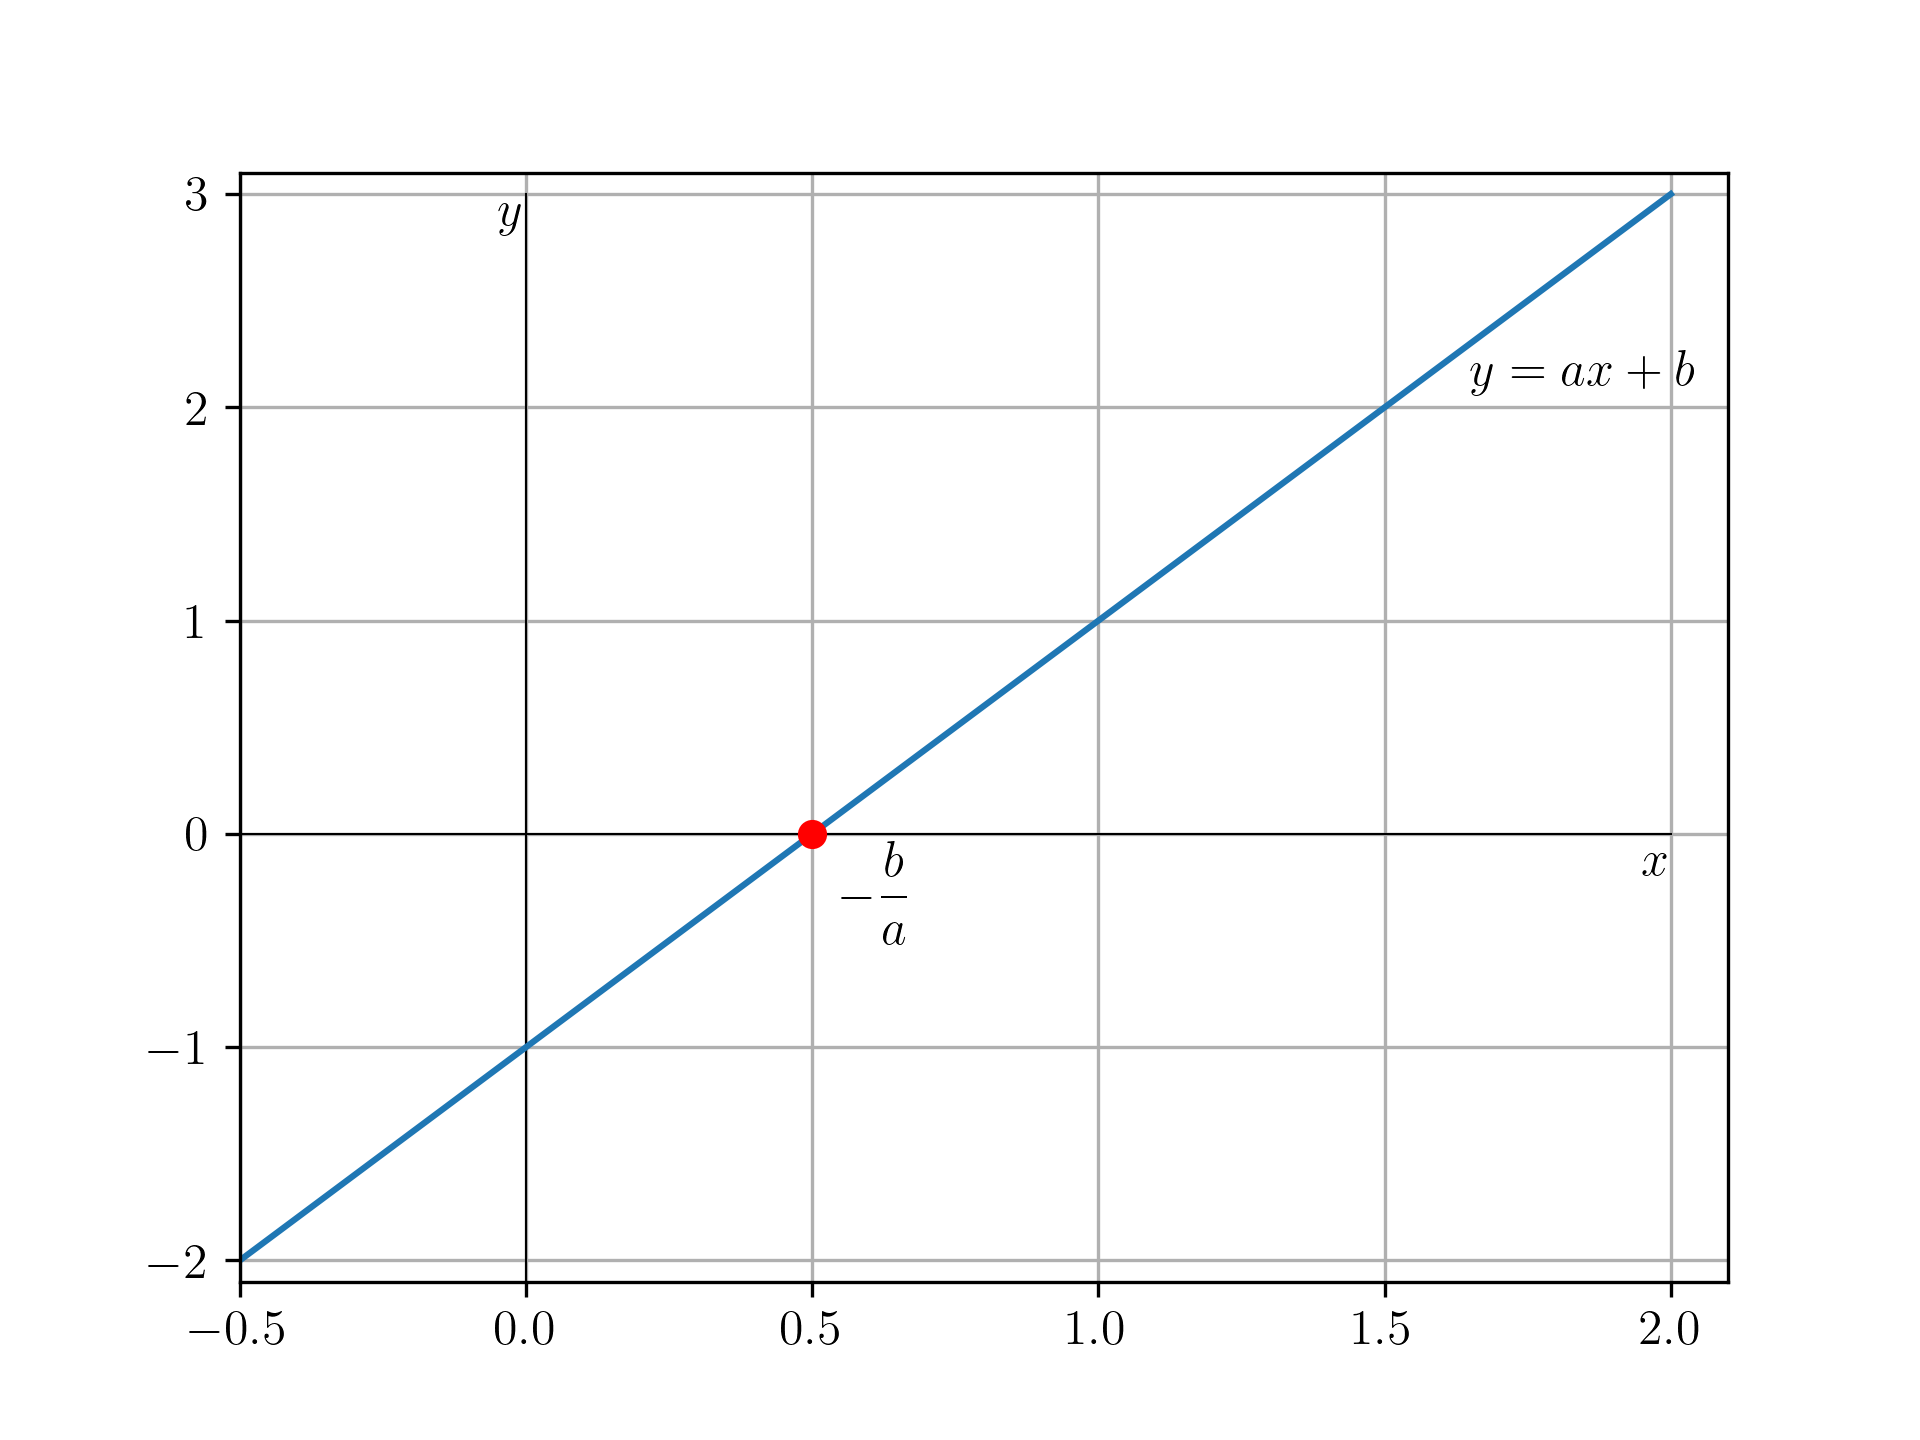
\includegraphics[max width=0.9\textwidth, height=2.75in]{./cap_lingua/dados/fig_ex_reta/fig.png}
    \caption{Esboço da reta de equação $y = ax + b$, com $a=2$ e $b=-1$.}
    \label{cap_lingua_sec_dados:fig:ex_reta}
  \end{figure}

  O ponto $x$ em que a reta intercepta o eixo das abscissas é
  \begin{equation}
    x = -\frac{b}{a}
  \end{equation}
  Assumindo que $a=2$ e $b=-1$, segue um algoritmo para a computação.
  \begin{enumerate}
  \item Atribuir o valor do \emph{coeficiente angular}
    \begin{equation}
      a\leftarrow 2.
    \end{equation}
  \item Atribuir o valor do \emph{coeficiente linear}
    \begin{equation}
      b\leftarrow -1.
    \end{equation}
  \item Computar e armazenar o valor do \emph{ponto de interseção com o eixo $x$}
    \begin{equation}
      x \leftarrow -\frac{b}{a}.
    \end{equation}
  \item Imprimir o valor de $x$.
  \end{enumerate}

  No algoritmo acima, os identificadores utilizados foram: $a$ para o \emph{coeficiente angular}, $b$ para o \emph{coeficiente linear} e $x$ para o \emph{ponto de interseção com o eixo x}.
\end{ex}


\hl{Em {\python}, os identificadores são sensíveis a letras maiúsculas e minúsculas (em inglês, \textit{case sensitive})}, i.e. o identificador \texttt{nome} é diferente dos \texttt{Nome}, \texttt{NoMe} e \texttt{NOME}. Por exemplo:

\begin{lstlisting}
>>> a = 7
>>> print(A)
Traceback (most recent call last):
  File "<stdin>", line 1, in <module>
NameError: name 'A' is not defined. Did you mean: 'a'?
\end{lstlisting}

\hl{Para melhorar a legibilidade de seus códigos, recomenda-se utilizar identificadores com nomes compostos} que ajudem a lembrar o significado do dado a que se referem. No exemplo acima (Exemplo~\ref{cap_lingua_sec_dados:ex:reta}), $a$ representa o \emph{coeficiente angular} da reta e um identificar apropriado seria \texttt{coefAngular} ou \texttt{coef\_angular}.

\hl{Identificadores não podem conter caracteres especiais} (\lstinline+*+, \lstinline+&+, \lstinline+%+,
\lstinline+@+, etc.), \hl{espaços em branco e começar com número}. As seguintes convenções para identificadores com nomes compostos são recomendadas:
\begin{itemize}
\item \hlemph{lowerCamelCase}: \texttt{nomeComposto}
\item \hlemph{UpperCamelCase}: \texttt{NomeComposto}
\item \hlemph{snake}: \texttt{nome\_composto}
\end{itemize}

\begin{obs}\normalfont{(\hl{Identificadores Reservados}.)}
  As seguintes palavras-chave (\texttt{keywords}) são identificadores pré-definidos e reservados:

\begin{verbatim}
  False   await     else     import    pass
  None    break     except   in        raise
  True    class     finally  is        return
  and     continue  for      lambda    try
  as      def       from     nonlocal  while
  assert  del       global   not       with
  async   elif      if       or        yield
\end{verbatim}

\end{obs}

\begin{ex}
  O algoritmo construído no Exemplo~\ref{cap_lingua_sec_dados:ex:reta} pode ser implementado como segue:

\begin{lstlisting}
coefAngular = 2
coefLinear = -1
intercepEixoX = -coefLinear/coefAngular
print(intercepEixoX)
\end{lstlisting}

\end{ex}

\subsection{Alocação de Dados}

Como estudamos acima, \hl{alocamos e referenciamos dados na memória do computador usando identificadores}. Em {\python}, ao executarmos a instrução

\begin{lstlisting}
x = 1
\end{lstlisting}

estamos alocando, na memória do computador, um \emph{objeto} com valor $1$ e \texttt{x} é uma referência para este dado. Pode-se imaginar a memória computacional como um sequência de caixinhas, de forma que \lstinline+x+ será a identificação da caixinha onde o valor $1$ foi alocado.

\begin{center}
  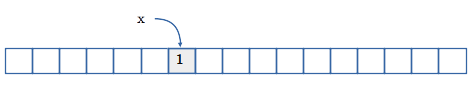
\includegraphics[width=4.5in]{./cap_lingua/dados/fig_aloc_mem/xRecebe1.png}
\end{center}

\hl{Em {\python}, dados têm identidades próprias}. Assim, quando executamos a instrução

\begin{lstlisting}
y = x 
\end{lstlisting}

o identificador \lstinline+y+ passa a referenciar o mesmo local de memória de \lstinline+x+.

\begin{center}
  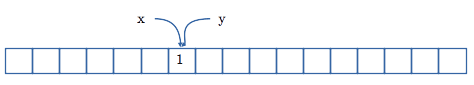
\includegraphics[width=4.5in]{./cap_lingua/dados/fig_aloc_mem/yRecebex.png}
\end{center}

Na sequência, se atribuirmos um novo valor para \lstinline+x+

\begin{lstlisting}
x = 2
\end{lstlisting}

este será alocado em um novo local na memória e \lstinline+x+ passa a referenciar este novo local.

\begin{center}
  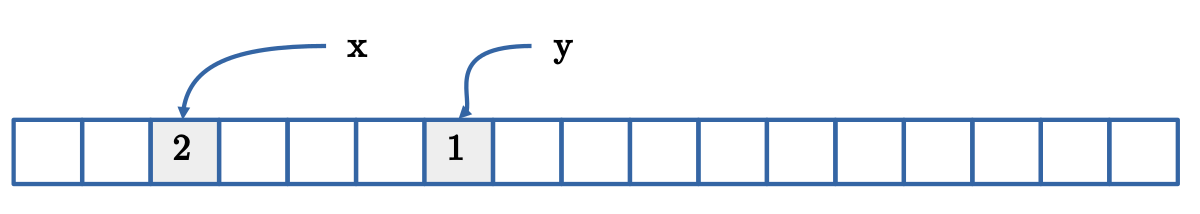
\includegraphics[width=4.5in]{./cap_lingua/dados/fig_aloc_mem/xRecebe2.png}
\end{center}

Ainda, se atribuirmos um novo valor para \lstinline+y+

\begin{lstlisting}
y = 3
\end{lstlisting}

este será alocado em um novo local na memória e \lstinline+y+ passa a referenciar este novo local. O local de memória antigo, em que o valor $1$ está alocado, passa a ficar novamente disponível para o sistema operacional.

\begin{center}
  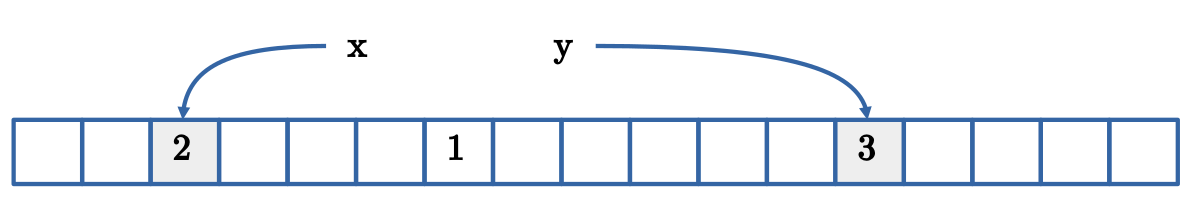
\includegraphics[width=4.5in]{./cap_lingua/dados/fig_aloc_mem/yRecebe3.png}
\end{center}

\begin{obs}
  O método {\python} {\PYTHONid} retorna a identidade de um objeto, seu registro único e constante durante sua alocação no código.

\begin{lstlisting}
x = 1
print('id(x) =', id(x))
\end{lstlisting}

\begin{verbatim}
id(x) = 139779845161200
\end{verbatim}

\begin{lstlisting}
y = x
print('id(y) =', id(y))
\end{lstlisting}

\begin{verbatim}
id(y) = 139779845161200
\end{verbatim}

\begin{lstlisting}
x = 2
print('id(x) =', id(x))
print('id(y) =', id(y))
\end{lstlisting}

\begin{verbatim}
id(x) = 139779845161232
id(y) = 139779845161200
\end{verbatim}

\begin{lstlisting}
y = 3
print('id(y) =', id(y))
\end{lstlisting}

\begin{verbatim}
id(y) = 139779845161264
\end{verbatim}


\end{obs}

\begin{ex}\normalfont{(\hl{Permutação de Variáveis/Identificadores}.)}\label{cap_lingua_sec_dados:ex:trocaVar}
Em várias situações, faz-se necessário permutar dados entre dois identificadores. Sejam

\begin{lstlisting}
x = 1
y = 2
\end{lstlisting}

Agora, queremos permutar os dados, ou seja, queremos que \texttt{y} tenha o valor $1$ e \texttt{x} o valor $2$. Podemos fazer isso utilizando uma variável auxiliar (em inglês, \textit{buffer}).

\begin{lstlisting}
z = x
x = y
y = z
\end{lstlisting}

Verifique!
\end{ex}

\subsection{Exercícios}

\begin{exer}
  Complete as lacunas.
  \begin{enumerate}[a)]
    % a)
    \item Programas de computadores processam, manipulam e organizam \underline{\phantom{dados}}.
    % b)
    \item Um \underline{\phantom{identificador}} é o nome atribuído para a identificação inequívoca de dados em um código computacional.
    % c)
    \item Objetos de um programa que armazenam dados que podem mudar de valor durante a execução do código são chamados de \underline{\phantom{variáveis}}.
    % d)
    \item Objetos que não mudam de valor durante a execução do código são chamados de \underline{\phantom{constantes}}.
    % e)
    \item \underline{\phantom{Função/método}} é um subprograma definido e executado em um programa.
  \end{enumerate}
\end{exer}
\begin{resp}
  a) dados. b) identificador. c) variáveis. d) constantes. e) função/método.
\end{resp}

\begin{exer}
  Proponha identificadores adequados à linguagem {\python} baseados nos seguintes nomes:
  \begin{enumerate}[a)]
  \item Área
  \item Perímetro do quadrado
  \item Cateto+Cateto
  \item Número de elementos do conjunto A
  \item 77 lados
  \item $f(x)$
  \item $x^2$
  \item $13x$
  \end{enumerate}
\end{exer}
\begin{resp}
  a) \lstinline+area+; b) \lstinline+perimetroQuad+; c) \lstinline+somaCatetos+; d) \lstinline+numElemA+; e) \lstinline+lados77+; f) \lstinline+fx+; g) \lstinline+x2+; h) \lstinline+xv13+
\end{resp}

\begin{exer}
  No Exemplo~\ref{cap_lingua_sec_algoprog:ex:areaTriang}, apresentamos um código {\python} para o cálculo da área de um triângulo. Reescreva o código trocando seus identificadores por nomes mais adequados.
\end{exer}
\begin{resp}

\begin{lstlisting}
base = float(input('Informe o valor da base.\n'))
altura = float(input('Informe o valor da altura.\n'))
# cálculo da área
area = base * altura /2
print(f'Área = {area}')
\end{lstlisting}

\end{resp}

\begin{exer}
  O seguinte código {\python} tem um erro/\textit{bug}:

\begin{lstlisting}
x = 1
y = X + 1
\end{lstlisting}

  Identifique-o e apresente uma nova versão do código corrigido.
\end{exer}
\begin{resp}
  Erro: variável \texttt{X} não foi definida.

\begin{lstlisting}
x = 1
y = x + 1
\end{lstlisting}

\end{resp}

\begin{exer}
  Faça uma representação gráfica da alocação de memória que ocorre para cada uma das instruções {\python} que seguem:

\begin{lstlisting}
x = 1
y = 2
z = x
x = y
y = z
\end{lstlisting}

\end{exer}
\begin{resp}

  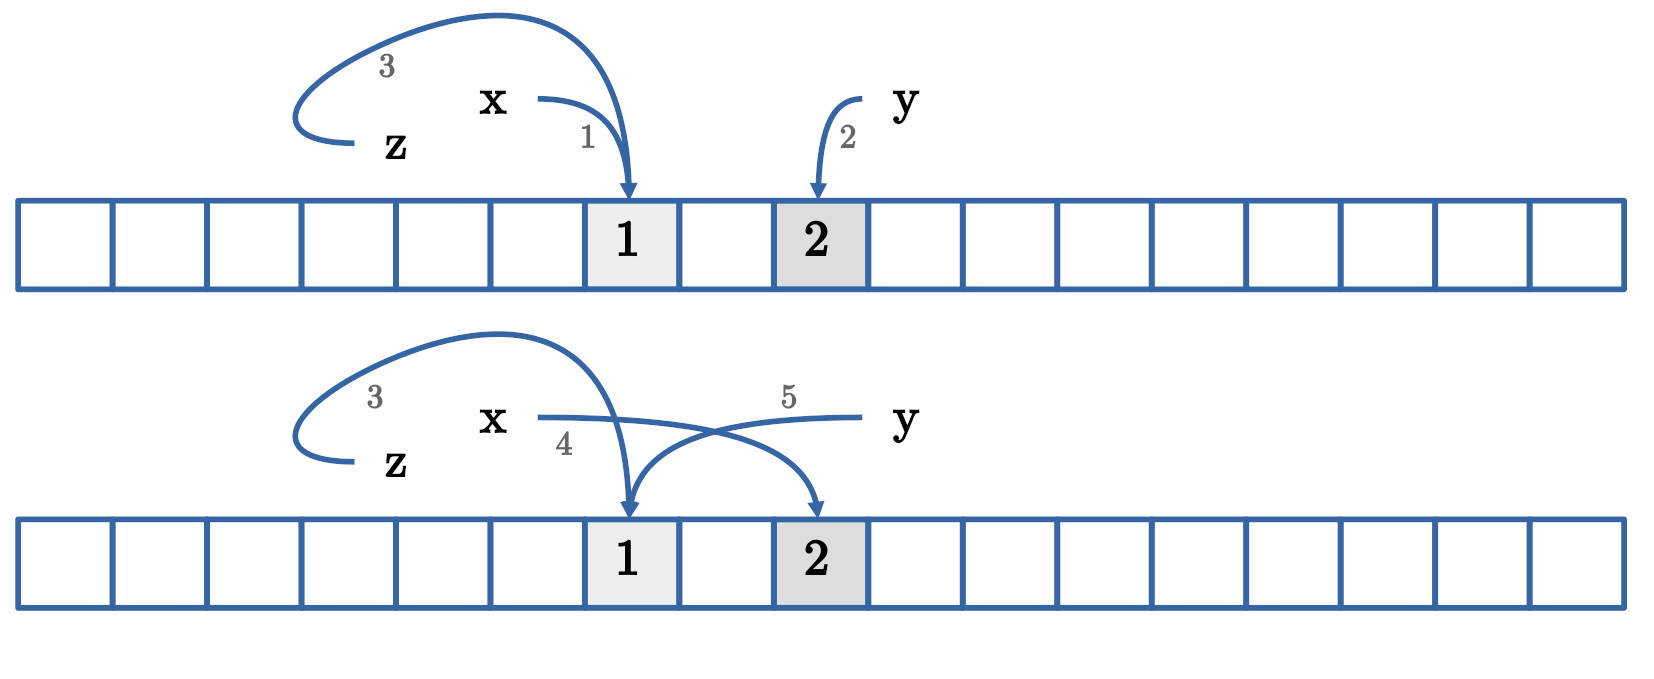
\includegraphics[width=4.5in]{./cap_lingua/dados/fig_aloc_mem/exerPermutacao.jpg}

\end{resp}

\begin{exer}
  No Exemplo~\ref{cap_lingua_sec_dados:ex:trocaVar} fazemos a permutação entre as variáveis \lstinline+x+ e \lstinline+y+ usando um \textit{buffer} \lstinline+z+ para guardar o valor de \lstinline+x+. Se, ao contrário, usarmos o \textit{buffer} para guardar o valor de \lstinline+y+, como fica o código de permutação entre as variáveis?
\end{exer}
\begin{resp}

\begin{lstlisting}
x = 1
y = 2
z = y
y = x
x = z
\end{lstlisting}

\end{resp}

\ifisbook
\subsubsection{Respostas}
\shipoutAnswer
\fi

\section{Dados Numéricos e Operações}\label{cap_lingua_sec_numop}

Números são tipos de dados usualmente manipulados \hl{em programas de computador}. \hl{Números inteiros e não inteiros são tratados de forma diferente}. Mas, antes de discorrermos sobre essas diferenças, vamos estudar operadores numéricos básicos.

\subsubsection{Operações Numéricas Básicas}

As seguintes operações numéricas estão disponíveis na linguagem {\python}:
\begin{itemize}
\item \lstinline*+* \hlemph{adição}

\begin{lstlisting}[xrightmargin=2.5em]
1 + 2
\end{lstlisting}

\begin{verbatim}
3
\end{verbatim}

\item \lstinline+-+ \hlemph{subtração}

\begin{lstlisting}[xrightmargin=2.5em]
1 - 2
\end{lstlisting}

\begin{verbatim}
-1
\end{verbatim}

\item \lstinline+*+ \hlemph{multiplicação}

\begin{lstlisting}[xrightmargin=2.5em]
2*3
\end{lstlisting}

\begin{verbatim}
6
\end{verbatim}

\item \lstinline+/+ \hlemph{divisão}

\begin{lstlisting}[xrightmargin=2.5em]
5/2
\end{lstlisting}

\begin{verbatim}
2.5
\end{verbatim}

\item \lstinline+**+ \hlemph{potenciação}

\begin{lstlisting}[xrightmargin=2.5em]
2**3
\end{lstlisting}

\begin{verbatim}
8
\end{verbatim}

\item \lstinline+//+ \hlemph{divisão inteira}

\begin{lstlisting}[xrightmargin=2.5em]
5//2
\end{lstlisting}

\begin{verbatim}
2
\end{verbatim}

\item \texttt{\%} \hlemph{resto da divisão}

\begin{lstlisting}[xrightmargin=2.5em]
5 % 2
\end{lstlisting}

\begin{verbatim}
1
\end{verbatim}

\end{itemize}

A \hlemph{ordem de precedência das operações} deve ser observada em {\python}. \hl{Uma expressão é executada da esquerda para a direita, mas os operadores tem a seguinte precedência}\footnote{Consulte na \textit{web} a lista completa de operadores e suas precedências em \href{https://docs.python.org/3/reference/expressions.html\#operator-precedence}{The Python Standard Library: Expressions: Operator precedence}.}:

\begin{enumerate}
\item \lstinline+**+
\item \lstinline*-x* (oposto de \texttt{x})
\item \lstinline+*, /, //, %+
\item \lstinline*+, -*
\end{enumerate}

\hl{Utilizamos parênteses para impor uma precedência diferente}, i.e. expressões entre parênteses \lstinline+()+ são executadas antes das demais.

\begin{ex}
  Estudamos a seguinte computação:

\begin{lstlisting}
2+8*3/2**2-1
\end{lstlisting}

\begin{verbatim}
7.0
\end{verbatim}

  Uma pessoa desavisada poderia pensar que o resultado está errado, pois
  \begin{align}
    &2+8 = 10,\\
    &10 \cdot 3 = 30,\\
    &30 \div 2 = 15,\\
    &15^2 = 225,\\
    &225 - 1 = 224.
  \end{align}
  Ou seja, o resultado não deveria ser $224$? Não, em {\python}, a operação de potenciação \lstinline+**+ tem a maior precedência, depois vem as de multiplicação \lstinline+*+ e divisão \lstinline+/+ (com a mesma precedência, sendo que a mais a esquerda é executada primeiro) e, por fim, vem as de adição \lstinline*+* e subtração \lstinline+-+ (também com a mesma precedência entre si). Ou seja, a instrução acima é computada na seguinte ordem:
  \begin{align}
    &2^2 = 4,\\
    &8\cdot 3 = 24,\\
    &24\div 4 = 6,\\
    &2 + 6 = 8,\\
    &8 - 1 = 7.
  \end{align}

  Para impormos uma ordem diferente de precedência, usamos parêntese. No caso acima, escrevemos

\begin{lstlisting}
((2 + 8)*3/2)**2 - 1
\end{lstlisting}

\begin{verbatim}
224.0
\end{verbatim}

\end{ex}

\begin{obs}\normalfont{(\hl{Espaços entre Operandos}.)}
  O uso de espaços entre os operandos, em geral, é arbitrário, mas conforme utilizados podem dificultar a legibilidade do código. Por exemplo,
\begin{lstlisting}
2 *- 3 + 2
\end{lstlisting}

\begin{verbatim}
-4
\end{verbatim}

  Essa expressão é computada na seguinte ordem
  \begin{align}
    &-~3 = -3\\
    &2\cdot(-3) = -6\\
    &-6 + 2 = -4.
  \end{align}
  Observamos que ela seria melhor escrita da seguinte forma

\begin{lstlisting}
2*-3 + 2
\end{lstlisting}

\begin{verbatim}
-4
\end{verbatim}

\end{obs}

\subsection{Números Inteiros}

\hl{Em {\python}, números inteiros são alocados por registros com um número arbitrário de \textit{bits}}. Com isso, os maior e menor números inteiros que podem ser alocados dependem da capacidade de memória da máquina. \hl{Quanto maior ou menor o número inteiro, mais \textit{bits} são necessários para alocá-lo}.

\begin{ex}
  O método {\python} {\PYTHONsysDOTgetsizeof} retorna o tamanho de um objeto medido em \textit{bytes} \hl{($1~\textit{byte} = 8~\textit{bits}$)}.

\begin{lstlisting}
import sys
print('0:',sys.getsizeof(0),'B')
print('1:',sys.getsizeof(1),'B')
print('100:',sys.getsizeof(100),'B')
print('10**9:',sys.getsizeof(10**9),'B'))
print('10**10:',sys.getsizeof(10**10),'B'))
print('10**100:',sys.getsizeof(10**100),'B'))
\end{lstlisting}

\begin{verbatim}
0: 24 B
1: 28 B
100: 28 B
10**9: 28 B
10**10: 32 B
10**100: 72 B
\end{verbatim}

  O número \href{https://en.wikipedia.org/wiki/Googol}{googol} $10^{100}$ é um número grande\footnote{Por exemplo, o número total de partículas elementares em todo o universo observável é estimado em $10^{80}$. Fonte: \href{https://en.wikipedia.org/wiki/Eddington_number}{Wikipedia: Eddington number}.}, mas $72$~\textit{bytes} não necessariamente. Um computador com $4$~Gbytes\footnote{$1~\textit{Gbytes} = 1024~\textit{Mbytes}$, $1~\textit{Mbytes} = 1024~\textit{Kbytes}$, $1~\textit{Kbytes} = 1024~\textit{bytes}$.} livres de memória, poderia armazenar um número inteiro que requer um registro de até $4,3\times 10^9~\textit{bytes}$.
\end{ex}

\begin{obs}
  O método {\python} {\PYTHONtype} retorna o tipo de objeto alocado. Números inteiros são objetos da classe {\PYTHONint}.

\begin{lstlisting}
type(10)
\end{lstlisting}

\begin{verbatim}
<class 'int'>
\end{verbatim}

\end{obs}

\subsection{Números Decimais}\label{cap_lingua_sec_numop:subsec:float}

No {\python}, \hl{números decimais são alocados} pelo padrão \href{https://en.wikipedia.org/wiki/IEEE\_754}{IEEE 774} de aritmética \hl{em ponto flutuante}. Em geral, são usados $64~\textit{bits} = 8~\textit{bytes}$ para alocar um número decimal. Um ponto flutuante tem a forma
\begin{equation}\hleq
  x = \pm m\cdot 2^{c-1023},
\end{equation}
onde $m\in [1,2)$ é chamada de mantissa e $c\in [0, 2047]$ é um número inteiro chamado de característica do ponto flutuante. A mantissa usa $52~\textit{bits}$, a característica $11~\text{bits}$ e $1~\textit{bit}$ é usado para o sinal do número.

\begin{lstlisting}
import sys
sys.float_info
\end{lstlisting}

\begin{verbatim}
sys.float_info(max=1.7976931348623157e+308, 
              max_exp=1024, 
              max_10_exp=308, 
              min=2.2250738585072014e-308, 
              min_exp=-1021, 
              min_10_exp=-307, 
              dig=15, 
              mant_dig=53, 
              epsilon=2.220446049250313e-16, 
              radix=2, 
              rounds=1)
\end{verbatim}

Vamos denotar \texttt{fl(x)} o número em ponto flutuante mais próximo do número decimal \texttt{x} dado. Quando digitamos

\begin{lstlisting}
x = 0.1
\end{lstlisting}

\hl{O valor alocado na memória da máquina não é \texttt{0.1}, mas, sim, o valor de \texttt{fl(x)}}. Normalmente, o \hlemph{épsilon de máquina} $\varepsilon = 2,22\times 10^{-16}$ é uma boa \hl{aproximação para o erro\footnote{Erro relativo.} (de arredondamento) entre \texttt{x} e \texttt{fl(x)}}.

\subsubsection{Notação Científica}

A \hl{\emph{notação científica}} é a representação de um dado número na forma
\begin{equation}
  d_{n}\ldots d_2d_1d_0,d_{-1}d_{-2}d_{-3}\ldots \times 10^{E},
\end{equation}
onde $d_i$, $i=n, \ldots, 1, 0, -1, \ldots$, são algarismos da base 10. A parte à esquerda do sinal $\times$ é chamada de \emph{mantissa} do número e $E$ é chamado de \emph{expoente} (ou ordem de grandeza).

\begin{ex}\label{cap_lingua_sec_numop:ex:notacao_cientifica}
  O número $31,415$ pode ser representado em notação científica das seguintes formas
  \begin{align}
    31,415\times 10^0 &= 3,1415\times 10^{1} \\
                      &= 314,15\times 10^{-1} \\
                      &= 0,031415\times 10^{3},
  \end{align}
  entre outras tantas possibilidades.

  \hl{Em {\python}, usa-se a letra \texttt{e} para separar a mantissa do expoente na notação científica}. Por exemplo

\begin{lstlisting}
# 31.415 X 10^0
31.415e0  
\end{lstlisting}

\begin{verbatim}
  31.515
\end{verbatim}

\begin{lstlisting}
# 314.15 X 10^-1
314.15e-1
\end{lstlisting}  

\begin{verbatim}
31.515  
\end{verbatim}

\begin{lstlisting}
# 0.031415 X 10^3
0.031415e3    
\end{lstlisting}

\begin{verbatim}
31.515  
\end{verbatim}
  
\end{ex}

No exemplo anterior (Exemplo~\ref{cap_lingua_sec_numop:ex:notacao_cientifica}), podemos observar que a representação em notação científica de um dado número não é única. Para contornar isto, introduzimos a \hl{\emph{notação científica normalizada}}, a qual tem a forma
\begin{equation}
  d_0,d_{-1}d_{-2}d_{-3}\ldots\times 10^{E},
\end{equation}
com $d_0 \neq 0$\footnote{No caso do número zero, temos $d_0=0$.}.

\begin{ex}
  O número $31,415$ representado em notação científica normalizada é $3,1415\times 10^{1}$.

  Em {\python}, podemos usar de especificação de formatação\footnote{Consulte Subseção~\ref{cap_lingua_sec_string:subsec:format} para mais informações.} para imprimir um número em notação científica normalizada. Por exemplo, temos

\begin{lstlisting}
x = 31.415
print(f'{x:e}')
\end{lstlisting}

\begin{verbatim}
3.141500e+01
\end{verbatim}

\end{ex}

\subsection{Números Complexos}

\hl{{\python} tem números complexos como uma classe básica da linguagem}. O número imaginário $i := \sqrt{-1}$ é representado por \texttt{1j}. Temos

\begin{lstlisting}
1j**2
\end{lstlisting}

\begin{verbatim}
(-1+0j)
\end{verbatim}

Ou seja, $i^2 = -1 + 0i$. \hl{Aritmética de números completos está diretamente disponível na linguagem}.

\begin{ex}
  Estudamos os seguintes casos:
  \begin{enumerate}[a)]
  \item $-3i + 2i = -i$

\begin{lstlisting}[framexrightmargin=-1.5em]
-3j + 2j
\end{lstlisting}

\begin{verbatim}
-1j
\end{verbatim}

  \item $(2 - 3i) + (4 + i) = 6 -2i$

\begin{lstlisting}[framexrightmargin=-1.5em]
2-3j + 4+1j
\end{lstlisting}

\begin{verbatim}
(6-2j)
\end{verbatim}

  \item $(2 - 3i)\cdot (4 + i) = 11 - 10i$

\begin{lstlisting}[framexrightmargin=-1.5em]
(2-3j)*(4+1j)
\end{lstlisting}

\begin{verbatim}
(11-10j)
\end{verbatim}

\end{enumerate}

\end{ex}

\subsection{Exercícios}

\begin{exer}
  Complete as lacunas.
  \begin{enumerate}[a)]
    % a)
    \item \underline{\phantom{\texttt{**}}} é o operador de potenciação.
    % b)
    \item A computação \texttt{2+2*3} resulta \underline{\phantom{\texttt{8}}}.
    % c)
    \item A computação \texttt{10-6/2} resulta \underline{\phantom{\texttt{7}}}.
    % d)
    \item A computação \texttt{3**2*3} resulta \underline{\phantom{\texttt{27}}}.
    % e)
    \item A computação \texttt{1-34/2*3} resulta \underline{\phantom{\texttt{50}}}.
  \end{enumerate}
\end{exer}
\begin{resp}
  a) \texttt{**}. b) \texttt{8}. c) \texttt{7}. d) \texttt{27}. e) \texttt{50}.
\end{resp}

\begin{exer}
  Desenvolva um código {\python} para computar a interseção com o eixo das abscissas da reta de equação
  \begin{equation}
    y =  2ax - b.
  \end{equation}
  Em seu código, aloque $a=2$ e $b=8$ e então compute o ponto de interseção $x$. Em seguida, teste seu código com outros valores possíveis de $a$ e $b$.
\end{exer}
\begin{resp}

\begin{lstlisting}
a = 2
b = 8
x = b/(2*a)
print("x = ", x)
\end{lstlisting}

\end{resp}

\begin{exer}
  Assuma que o seguinte código {\python}

\begin{lstlisting}
a = 2
b = 8
x = b/2*a
print("x = ", x)
\end{lstlisting}

tenha sido desenvolvido para computar o ponto de interseção com o eixo das abscissas da reta de equação
  \begin{equation}
    y = 2ax - b
  \end{equation}
  com $a=2$ e $b=8$. O código acima contém um erro, qual é? Identifique-o, corrija-o e justifique sua resposta.
\end{exer}
\begin{resp}
  Erro na linha 3. As operações não estão ocorrendo na precedência correta para fazer a computação desejada. Correção: \lstinline+x = b/(2*a)+.
\end{resp}

\begin{exer}
  Desenvolva um código {\python} para computar a média aritmética entre dois números $x$ e $y$ dados. Teste seu código para diferentes valores de $x$ e $y$.
\end{exer}
\begin{resp}

\begin{lstlisting}
x = 3
y = 9
media = (x + y)/2
print('média = ', media)
\end{lstlisting}

\end{resp}

\begin{exer}
  Uma disciplina tem o seguinte critério de avaliação:
  \begin{enumerate}
  \item Trabalho: nota com peso 3.
  \item Prova: nota com peso 7.
  \end{enumerate}
  Desenvolva um código {\python} que compute a nota final, dadas as notas do trabalho e da prova (em escala de $0 - 10$) de um estudante. Teste seu código para diferentes valores de notas.
\end{exer}
\begin{resp}

\begin{lstlisting}
notaTrabalho = 8.5
notaProva = 7
notaFinal = (notaTrabalho*3 + notaProva*7)/10
print('Nota final = ', notaFinal)
\end{lstlisting}

\end{resp}

\begin{exer}
  Desenvolva um código {\python} para computar as raízes reais de uma equação quadrática
  \begin{equation}
    ax^2 + bx + c = 0.
  \end{equation}
  Assuma dados os parâmetros $a=2$, $b=-2$ e $c=-12$. Em seguida, teste seu código para diferentes valores dos parâmetros $a$, $b$ e $c$.
\end{exer}
\begin{resp}

\begin{lstlisting}
a = 2
b = -2
c = -12
delta = b**2 - 4*a*c
x1 = (-b - delta**(1/2))/(2*a)
print('x1 = ', x1)
x2 = (-b + delta**(1/2))/(2*a)
print('x2 = ', x2)
\end{lstlisting}

\end{resp}

\begin{exer}
  Encontre a quantidade de memória disponível em seu computador. Quantos números decimais em ponto flutuante de $64$-\textit{bits} seu programa poderia alocar, caso conseguisse usar toda a memória disponível no momento?
\end{exer}
\begin{resp}
  Cada $1$ \texttt{GBytes} livre permite alocar aproximadamente $10^8$ números decimais.
\end{resp}

\begin{exer}
  Escreva os seguintes números em notação científica normalizada e entre com eles em um terminal {\python}:
  \begin{enumerate}[a)]
  \item $700$
  \item $0,07$
  \item $2800000$
  \item $0,000019$
  \end{enumerate}
\end{exer}
\begin{resp}
  a) $7\times 10^2$, \lstinline+7e2+; b) $7\times 10^{-2}$, \lstinline+7e-2+; c) $2,8\times 10^6$, \lstinline+2.8e6+; d) $1.9\times 10^{-5}$, \lstinline+1.9e-5+
\end{resp}

\begin{exer}
  Escreva os seguintes números em notação decimal:
  \begin{enumerate}
  \item $2,8\times 10^{-3}$
  \item $8,712\times 10^4$
  \item $3,\overline{3}\times 10^{-1}$
  \end{enumerate}
\end{exer}
\begin{resp}
  a) $0.0028$; b) $87120$; c) $0,\overline{3}$
\end{resp}

\begin{exer}
  Faça os seguintes cálculos e, então, verifique os resultados computando-os em {\python}:
  \begin{enumerate}
  \item $5\times 10^{3} + 3\times 10^{2}$
  \item $8,1\times 10^{-2} - 1\times 10^{-3}$
  \item $\left(7\times 10^4\right)\cdot (2\times 10^{-2})$
  \item $\left(7\times 10^{-4}\right)\div (2\times 10^{2})$
  \end{enumerate}
\end{exer}
\begin{resp}
  a) $5,3\times 10^3$;

\begin{lstlisting}
x = 5e3 + 3e2
print(f'{x:e}')
\end{lstlisting}
  
  b) $8\times 10^{-2}$

\begin{lstlisting}
x = 8.1e-2 - 1e-3
print(f'{x:e}')
\end{lstlisting}

  c) $1,4\times 10^{3}$

\begin{lstlisting}
x = 7e4 * 2e-2
print(f'{x:e}')
\end{lstlisting}

  d) $3,5\times 10^{-6}$

\begin{lstlisting}
x = 7e-4 / 2e2
print(f'{x:e}')
\end{lstlisting}

\end{resp}


\begin{exer}
  Faça os seguintes cálculos e verifique seus resultados computando-os em {\python}:
  \begin{enumerate}
  \item $(2-3i) + (2-i)$
  \item $(1+2i) - (1-3i)$
  \item $(2-3i) \cdot (-4+2i)$
  \item $(1-i)^3$
  \end{enumerate}
\end{exer}
\begin{resp}
  a) $3+7i$

\begin{lstlisting}
(1+8j) + (2-1j)
\end{lstlisting}

  b) $5i$

\begin{lstlisting}
(1+2j) - (1-3j)
\end{lstlisting}

  c) $-2+16i$

\begin{lstlisting}
(2-3j) * (-4+2j)
\end{lstlisting}

  d) $-2-2i$

\begin{lstlisting}
(1-1j)**3
\end{lstlisting}

\end{resp}


\begin{exer}
  Desenvolva um código {\python} que computa a área de um quadrado de lado $l$ dado. Teste-o com $l=0,575$ e assegure que seu código forneça o resultado usando notação científica.
\end{exer}
\begin{resp}

\begin{lstlisting}
lado = 0.575
area = lado**2
print(f'área = {area:e}')
\end{lstlisting}

\end{resp}

\begin{exer}
  Desenvolva um código {\python} que computa o comprimento da diagonal de um quadrado de lado $l$ dado. Teste-o com $l=2$ e assegure que seu código forneça o resultado em notação científica normalizada.
\end{exer}
\begin{resp}

\begin{lstlisting}
lado = 2
diag = lado*2**(1/2)
print(f'diagonal = {diag:e}')
\end{lstlisting}

\end{resp}

\begin{exer}
  Assumindo que $a_1\neq a_2$, desenvolva um código {\python} que compute o ponto $(x_{i}, y_i)$ que corresponde a interseção das retas de equações
  \begin{align}
    &y = a_1x + b_1\\
    &y = a_2x + b_2,
  \end{align}
  para $a_1$, $a_2$, $b_1$ e $b_2$ parâmetros dados. Teste-o para o caso em que $a_1=1$, $a_2=-1$, $b_1=1$ e $b_2=-1$. Garanta que seu código forneça a solução usando notação científica normalizada.
\end{exer}
\begin{resp}

\begin{lstlisting}
# parâmetros
a1 = 1
a2 = -1
b1 = 1
b2 = -1
# ponto x de interseção
x_intercep = (b2-b1)/(a1-a2)
# ponto y de interceção
y_intercep = a1*x_intercep + b1
# imprime o resultado
print(f'x_i = {x_intercep:e}')
print(f'y_i = {y_intercep:e}')
\end{lstlisting}

\end{resp}

\ifisbook
\subsubsection{Respostas}
\shipoutAnswer
\fi

\section{Dados Booleanos}\label{cap_lingua_sec_bool}

Em {\python}, os \hl{\emph{valores lógicos} são o {\PYTHONTrue} (\emph{verdadeiro}) e o {\PYTHONFalse} (\emph{falso})}. Pertencem a uma subclasse dos números inteiros, com \lstinline+1+ correspondendo a {\PYTHONTrue} e \lstinline+0+ a {\PYTHONFalse}. Em referência ao matemático George Boole{\boole}, estes dados são chamados de \emph{booleanos}.

Normalmente, eles aparecem como resultado de expressões lógicas. Por exemplo:

\begin{lstlisting}
2/3 < 3/4
\end{lstlisting}

\begin{verbatim}
True
\end{verbatim}

\begin{lstlisting}
7/5 > 13/9
\end{lstlisting}

\begin{verbatim}
  False
\end{verbatim}

\subsection{Operadores de Comparação}

{\python} possui \hl{\emph{operadores de comparação}} que \hl{retornam valores lógicos}, são eles:
\begin{itemize}
\item \lstinline+<+ \hlemph{menor que}

\begin{lstlisting}[xrightmargin=2.5em]
2 < 3
\end{lstlisting}

\begin{verbatim}
True
\end{verbatim}

\item \lstinline+<=+ \hlemph{menor ou igual que}

\begin{lstlisting}[xrightmargin=2.5em]
4 <= 2**2
\end{lstlisting}

\begin{verbatim}
True
\end{verbatim}

\item \lstinline+>+ \hlemph{maior que}

\begin{lstlisting}[xrightmargin=2.5em]
5 > 7
\end{lstlisting}

\begin{verbatim}
False
\end{verbatim}

\item \lstinline+>=+ \hlemph{maior ou igual que}

\begin{lstlisting}[xrightmargin=2.5em]
2*5 >= 10
\end{lstlisting}

\begin{verbatim}
True
\end{verbatim}

\item \lstinline+==+ \hlemph{igual a}

\begin{lstlisting}[xrightmargin=2.5em]
9**2 == 81
\end{lstlisting}

\begin{verbatim}
True
\end{verbatim}

\item \lstinline+!=+ \hlemph{diferente de}

\begin{lstlisting}[xrightmargin=2.5em]
81 != 9**2
\end{lstlisting}

\begin{verbatim}
False
\end{verbatim}

\end{itemize}

\begin{obs}\normalfont{(\hl{Precedência de operações}.)}
  Os operadores de comparação \lstinline+<+, \lstinline+<=+, \lstinline+>+, \lstinline+>=+, \lstinline+==+, \lstinline+!=+ tem a mesma ordem de precedência e estão abaixo da precedência dos operadores numéricos básicos.
\end{obs}

\begin{ex}
  A equação da circunferência de centro no ponto $(a, b)$ e raio $r$ é
  \begin{equation}
    (x-a)^2 + (y-b)^2 = r^2.
  \end{equation}
  Um ponto $(x, y)$ está no disco determinado pela circunferência, quando
  \begin{equation}
    (x-a)^2 + (y-b)^2 \leq r^2
  \end{equation}
  e está fora do disco, noutro caso.

  O seguinte código verifica se o ponto dado $(x, y) = (1, 1)$ está no disco determinado pela circunferência de centro $(a, b) = (0, 0)$ e raio $r = 1$.

  
\begin{lstlisting}
# ponto
x = 1
y = 1

# centro circunferência
a = 0
b = 0
# raio circunferência
raio = 1

# verifica se está no disco
v = (x-a)**2 + (y-b)**2 <= raio**2

# imprime resposta
print('O ponto está no disco?', v)
\end{lstlisting}

\end{ex}

\subsubsection{Comparação entre Pontos Flutuantes}

\hl{Números decimais são arredondados para o número \PYTHONfloat (ponto flutuante) mais próximo na máquina}\footnote{Consulte a Subseção~\ref{cap_lingua_sec_numop:subsec:float} para mais informações.}. Com isso, a comparação direta entre pontos flutuantes não é recomendada, em geral. Por exemplo,

\begin{lstlisting}
0.1 + 0.2 == 0.3
\end{lstlisting}

\begin{verbatim}
False
\end{verbatim}

Inesperadamente, este resultado é esperado na aritmética de ponto flutuante! \lstinline+:)+

O que ocorre acima, é que ao menos um dos números (na verdade todos) não tem representação exata como ponto flutuante. Isso faz com que a soma \lstinline*0.1 + 0.2* não seja exatamente computada igual a \lstinline+0.3+.

O erro de arredondamento é de aproximadamente\footnote{Épsilon de máquina $\varepsilon \approx 2,22\times 10^{-16}$.} $10^{-16}$ para cada entrada. Conforme operamos sobre pontos flutuantes este erro pode crescer. Desta forma, \hl{o mais apropriado para comparar se dois pontos flutuantes são iguais (dentro do erro de arrendamento de máquina) é verificando se a distância entre eles é menor que uma precisão desejada}, por exemplo, $10^{-15}$. No caso acima, podemos usar o método {\PYTHONabs}:

\begin{lstlisting}
abs(x - 0.3) <= 1e-15
\end{lstlisting}

\begin{verbatim}
True
\end{verbatim}

\subsection{Operadores Lógicos}

{\python} tem os operadores lógicos (ou \hl{\emph{operadores booleanos}}):
\begin{itemize}
\item \lstinline+and+ \hlemph{\texttt{e} lógico}

\begin{lstlisting}[xrightmargin=2.5em]
3 > 4 and 3 <= 4
\end{lstlisting}

\begin{verbatim}
False
\end{verbatim}

  \begin{table}[H]
    \centering
    \caption{Tabela verdade do \lstinline+and+.}
    \begin{tabular}{ll|l}
      {\texttt{A}} & {\texttt{B}} & {\lstinline+A and B+}\\\hline
      {\texttt{True}} & {\texttt{True}} & {\texttt{True}}\\
      {\texttt{True}} & {\texttt{False}} & {\texttt{False}}\\
      {\texttt{False}} & {\texttt{True}} & {\texttt{False}}\\
      {\texttt{False}} & {\texttt{False}} & {\texttt{False}}\\\hline
    \end{tabular}
  \end{table}

\ifisbook
\newpage
\fi

\item \lstinline+or+ \hlemph{\texttt{ou} lógico}

\begin{lstlisting}[xrightmargin=2.5em]
3 > 4 or 3 <= 4
\end{lstlisting}

\begin{verbatim}
True
\end{verbatim}

  \begin{table}[H]
    \centering
    \caption{Tabela verdade do \lstinline+or+.}
    \begin{tabular}{ll|l}
      {\texttt{A}}     & {\texttt{B}}     & {\lstinline+A or B+} \\\hline
      {\texttt{True}}  & {\texttt{True}}  & {\texttt{True}} \\
      {\texttt{True}}  & {\texttt{False}} & {\texttt{True}} \\
      {\texttt{False}} & {\texttt{True} } & {\texttt{True}} \\
      {\texttt{False}} & {\texttt{False}} & {\texttt{False}} \\\hline
    \end{tabular}
  \end{table}

\item \lstinline+not+ \hlemph{negação lógica}

\begin{lstlisting}[xrightmargin=2.5em]
not(3 < 2)
\end{lstlisting}

\begin{verbatim}
True
\end{verbatim}

  \begin{table}[H]
    \centering
    \caption{Tabela verdade do \lstinline+not+.}
    \begin{tabular}{l|l}
      {\texttt{A}}     & {\lstinline+not A+} \\\hline
      {\texttt{True}}  & {\texttt{False}} \\
      {\texttt{False}} & {\texttt{True}} \\\hline
    \end{tabular}
  \end{table}  
\end{itemize}

\begin{obs}\normalfont{(\hl{Precedência de operações}.)}
  Os operadores booleanos tem a seguinte ordem de precedência:
  \begin{enumerate}[1.]
  \item \lstinline+not+
  \item \lstinline+and+
  \item \lstinline+or+
  \end{enumerate}
  São executados em ordem de precedência menor que os operadores de comparação.
\end{obs}

\begin{ex}
  Sejam os discos determinados pelas circunferências
  \begin{align}
    c_1&: (x - a_1)^2 + (y + b_1)^2 = r_1^2,\\
    c_2&: (x - a_2)^2 + (y + b_2)^2 = r_2^2,
  \end{align}
  onde $(a_1, b_1)$ e $(a_2, b_2)$ são seus centros e $r_1$ e $r_2$ seus raios, respectivamente.

  Assumindo, que a circunferência $c_1$ tem
  \begin{equation}
    c_1: (a_1, b_1) = (0, 0), r_1 = 1
  \end{equation}
  e a circunferência $c_2$ tem
  \begin{equation}
    c_2: (a_2, b_2) = (1, 1), r_2 = 1,
  \end{equation}
  o seguinte código verifica se o ponto $(x, y) = \left(\frac{1}{2}, \frac{1}{2}\right)$ pertence a interseção dos discos determinados por $c_1$ e $c_2$.

\begin{lstlisting}
# circunferência c1
a1 = 0
b1 = 0
r1 = 1

# circunferência c2
a2 = 1
b2 = 1
r2 = 1

# ponto obj
x = 0.5
y = 0.5

# está em c1?
em_c1 = (x-a1)**2 + (y-b1)**2 <= r1**2

# está em c2?
em_c2 = (x-a2)**2 + (y-b2)**2 <= r2**2

# está em c1 e c2?
resp = em_c1 and em_c2
print('O ponto está na interseção de c1 e c2?', resp)
\end{lstlisting}
\end{ex}

\ifisbook
\vspace{0.5cm}
\fi

\begin{obs}\normalfont{(\hl{Ou exclusivo}.)}\label{cap_lingua_sec_bool:obs:xor}
  Presente em algumas linguagens, {\python} não tem um operador \lstinline+xor+ (ou exclusivo). A tabela verdade do ou exclusivo é
  \begin{center}
    \begin{tabular}[H]{ll|l}
      {\texttt{A}}     & {\texttt{B}}     & {\lstinline+A xor B+} \\\hline
      {\texttt{True}}  & {\texttt{True}}  & {\texttt{False}}   \\
      {\texttt{True}}  & {\texttt{False}} & {\texttt{True}}    \\
      {\texttt{False}} & {\texttt{True}}  & {\texttt{True}}    \\
      {\texttt{False}} & {\texttt{False}} & {\texttt{False}}   \\\hline    
    \end{tabular}
  \end{center}
  \hl{A operação \texttt{xor} pode ser obtida através de expressões lógicas usando-se apenas os operadores \texttt{and}, \texttt{or} e \texttt{not}}. Consulte o Exercício~\ref{cap_lingua_sec_bool:exer:xor}.
\end{obs}

\subsection{Exercícios}

\begin{exer}
  Considerando a linguagem {\python}, complete as lacunas.
  \begin{enumerate}[a)]
    % a)
    \item \underline{\phantom{\texttt{True}}} é o valor lógico verdadeiro.
    % b)
    \item \texttt{False} é o valor lógico \underline{\phantom{falso}}.
    % c)
    \item O operador de igualdade é o \underline{\phantom{\texttt{==}}}.
    % d)
    \item \texttt{1.275 }\underline{\phantom{\texttt{!=}}}\texttt{ 1.275} retorna o valor booleano \texttt{False}.
  \end{enumerate}
\end{exer}
\begin{resp}
  a) \texttt{True}. b) falso. c) \texttt{==}. d) \texttt{!=}.
\end{resp}

\begin{exer}
  Sem implementar, complete as lacunas.
  \begin{enumerate}[a)]
    % a)
    \item \texttt{8 * 2 < 3} retorna o valor \underline{\phantom{\texttt{False}}}.
    % b)
    \item \texttt{2 * 8 > 9} retorna o valor \underline{\phantom{\texttt{True}}}.
    % c)
    \item \texttt{4 >= 3**2} retorna o valor \underline{\phantom{\texttt{False}}}.
    % d)
    \item \texttt{16 == 16 // 8} retorna o valor \underline{\phantom{\texttt{False}}}.
  \end{enumerate}
\end{exer}
\begin{resp}
  a) \texttt{False}.  b) \texttt{True}.  c) \texttt{False}. d) \texttt{False}.
\end{resp}

\begin{exer}
  Complete as lacunas.
  \begin{enumerate}[a)]
    % a)
    \item \texttt{True and }\underline{\phantom{\texttt{True}}} retorna o valor \texttt{True}.
    % b)
    \item \texttt{False or True} retorna o valor \underline{\phantom{\texttt{True}}}.
    % c)
    \item \texttt{not (5 > 3)} retorna o valor \underline{\phantom{\texttt{False}}}.
  \end{enumerate}
\end{exer}
\begin{resp}
  a) \texttt{True}. b) \texttt{True}. c) \texttt{False}.
\end{resp}

\begin{exer}
  Compute as seguintes expressões:
  \begin{enumerate}[a)]
  \item $1 - 6 > -6$
  \item $\frac{3}{2} < \frac{4}{3}$
  \item $31,415\times 10^{-1} == 3.1415$
  \item $\displaystyle 2,7128 \geq 2 + \frac{2}{3}$
  \item $\displaystyle \frac{3}{2} + \frac{7}{8} \leq \frac{24 + 14}{16}$
  \end{enumerate}
\end{exer}
\begin{resp}
  a) \lstinline+1 - 6 > -6+ b) \lstinline+3/2 < 4/3+ c) \lstinline+31.415e-1 == 3.1415+ d) \lstinline+2.7128 >= 2 + 2/3+ e) \lstinline+3/2 + 7/8 <= (24 + 14)/16+
\end{resp}

\begin{exer}
  Desenvolva um código que verifica se um número inteiro $x$ dado é par. Teste-o para diferentes valores de $x$.
\end{exer}
\begin{resp}

\begin{lstlisting}
x = 3
print('É par?')
print(x % 2 == 0)
\end{lstlisting}

\end{resp}

\begin{exer}
  Considere um quadrado de lado $l$ dado e uma circunferência de raio $r$ dado. Desenvolva um código que verifique se a área do quadrado é menor que a da circunferência. Teste o seu código para diferentes valores de $l$ e $r$.
\end{exer}
\begin{resp}

\begin{lstlisting}
# quadrado
ladoQuad = 1
areaQuad = ladoQuad**2

# aprox pi
pi = 3.14159

# circunferência
raioCirc = 1
areaCirc = pi * raioCirc**2

# verifica
resp = areaQuad < areaCirc
print('Área do quadrado é menor que da circunferência?')
print(resp)
\end{lstlisting}

\end{resp}

\begin{exer}
  Considere o plano cartesiano $x-y$. Desenvolva um código que verifique se um ponto $(x, y)$ dado está entre a curvas $y = (x-1)^3$ e o eixo das abscissas\footnote{Eixo $x$.}. Verifique seu código para diferentes pontos $(x, y)$.
\end{exer}
\begin{resp}

\begin{lstlisting}
# ponto
x = 2
y = 0.5

# y >= 0 e y <= f(x) ?
resp1 = y >= 0 and y <= (x-1)**3
# y >= f(x) e y <= 0 ?
resp2 = y >= (x-1)**3 and y <= 0

# conclusão
print("O ponto está entre as curvas?")
print(resp1 or resp2)
\end{lstlisting}

\end{resp}

\begin{exer}
  Sejam $A$ e $B$ valores booleanos. Verifique se as seguintes expressões são verdadeiras (\texttt{True}) ou falsas (\texttt{False}):
  \begin{enumerate}[a)]
  \item \lstinline+A or A == A+
  \item \lstinline+A and not(A) == True+
  \item \lstinline+A or (A and B) == A+
  \item \lstinline+not(A and B) == (not(A) or not(B))+
  \item \lstinline+not(A or B) == (not(A) or not(B))+
  \end{enumerate}
\end{exer}
\begin{resp}
  a) \texttt{True}. b) \texttt{False}. c) \texttt{True}. d) \texttt{True}. e) \texttt{False}.
\end{resp}

\begin{exer}\label{cap_lingua_sec_bool:exer:xor}
  Sejam \texttt{A} e \texttt{B} valores booleanos dados. Escreva uma expressão lógica que emule a operação \lstinline+xor+ (ou exclusivo) usando apenas os operadores \lstinline+and+, \lstinline+or+ e \lstinline+not+. Dica: consulte a Observação~\ref{cap_lingua_sec_bool:obs:xor}.
\end{exer}
\begin{resp}
  \lstinline+(A or B) and not(A and B)+
\end{resp}

\ifisbook
\subsubsection{Respostas}
\shipoutAnswer
\fi

\section{Sequência de Caracteres}\label{cap_lingua_sec_string}

Dados em formato texto também são comumente manipulados em programação. \hl{Um texto é interpretado como uma cadeia/\emph{sequência de caracteres}\footnote{Caractere é qualquer letra, símbolo, sinal ou dígito representado em forma escrita.}, chamada de \texttt{string}}. Para entrarmos com uma letra, palavra ou texto (uma \texttt{string}), precisamos usar aspas (simples \lstinline+' '+ ou duplas \lstinline+" "+). Por exemplo,

\begin{lstlisting}
s = 'Olá, mundo!'
print(s)
\end{lstlisting}

\begin{verbatim}
Olá, mundo!  
\end{verbatim}

\begin{lstlisting}
type(s)
\end{lstlisting}

\begin{verbatim}
<class 'str'>
\end{verbatim}

Uma \hl{\texttt{string} é um conjunto \emph{indexado} e \emph{imutável} de caracteres.} O primeiro caractere está na posição $0$, o segundo na posição $1$ e assim por diante. Por exemplo,
\begin{equation}
  \underset{0}{\texttt{O}}~\underset{1}{\texttt{l}}~\underset{2}{\texttt{á}}~\underset{3}{\texttt{,}}~\underset{4}{\texttt{\_}}~\underset{5}{\texttt{m}}~\underset{6}{\texttt{u}}~\underset{7}{\texttt{n}}~\underset{8}{\texttt{d}}~\underset{9}{\texttt{o}}~\underset{10}{\texttt{!}}
\end{equation}
Observamos que o espaço também é um caractere. O tamanho da \texttt{string} (número total de caracteres) pode ser obtido com o método {\PYTHONlen}, por exemplo

\begin{lstlisting}
len(s)
\end{lstlisting}

\begin{verbatim}
11
\end{verbatim}

A referência a um caractere de uma dada \texttt{string} é feito usando-se seu identificador seguido do índice de sua posição entre colchetes. Por exemplo,

\begin{lstlisting}
s[6]
\end{lstlisting}

\begin{verbatim}
'u'
\end{verbatim}

Podemos, ainda, \hl{acessar fatias}\footnote{Em inglês, \textit{slice}.}\hl{ da sequência usando o operador \texttt{:}}\footnote{{\lstinline+x[start:stop:step]+}, padrão {\lstinline+start=0+}, {\lstinline+stop=len(x)+}, {\lstinline+step=1+.}}, por exemplo,

\begin{lstlisting}
s[:3]
\end{lstlisting}

\begin{verbatim}
'Olá'
\end{verbatim}

ou seja, os caracteres da posição $0$ à posição $2$ (um antes do índice $3$). Também podemos tomar uma fatia entre posições, por exemplo,

\begin{lstlisting}
s[5:10]
\end{lstlisting}

\begin{verbatim}
'mundo'
\end{verbatim}

o que nos fornece a fatia de caracteres que inicia na posição $5$ e termina na posição $9$. Ou ainda,

\begin{lstlisting}
s[6:]
\end{lstlisting}

\begin{verbatim}
'undo!'
\end{verbatim}

Também, pode-se controlar o passo do fatiamento, por exemplo

\begin{lstlisting}
'laura'[::2]
\end{lstlisting}

\begin{verbatim}
'lua'
\end{verbatim}

Em {\python}, exitem diversas \hl{formas de escrever \texttt{strings}}:
\begin{itemize}
\item \hlemph{aspas simples}

\begin{lstlisting}[xrightmargin=2.5em]
print('permitem aspas "duplas" embutidas')
\end{lstlisting}

\begin{verbatim}
permitem aspas "duplas" embutidas
\end{verbatim}

\item \hlemph{aspas duplas}

\begin{lstlisting}[xrightmargin=2.5em]
print("permitem aspas 'simples' embutidas")
\end{lstlisting}

\begin{verbatim}
permitem aspas 'simples' embutidas
\end{verbatim}

\item \hlemph{aspas triplas}

\begin{lstlisting}[xrightmargin=2.5em]
print('''
permitem
"diversas"
linhas
''')
\end{lstlisting}

\begin{verbatim}
permitem
"diversas"
linhas  
\end{verbatim}

\begin{lstlisting}
print("""
permitem
'diversas'
linhas
""")
\end{lstlisting}

\begin{verbatim}
permitem
'diversas'
linhas  
\end{verbatim}
  
\end{itemize}

Em {\python}, \texttt{strings} usam o padrão \href{https://home.unicode.org/}{Unicode}, que permite manipular textos de forma muito próxima da linguagem natural. Alguns caracteres especiais úteis são:
\begin{itemize}
\item \lstinline+'\n'+ \hlemph{nova linha}

\begin{lstlisting}[xrightmargin=2.5em]
print('Uma nova\nlinha')
\end{lstlisting}

\begin{verbatim}
Uma nova
linha  
\end{verbatim}

\item \lstinline+'\t'+ \hlemph{tabulação}

\begin{lstlisting}[xrightmargin=2.5em]
print('Uma nova\n\t linha com tabulação')
\end{lstlisting}

\begin{verbatim}
Uma nova
  linha com tabulação
\end{verbatim}
\end{itemize}

\begin{obs}\normalfont{(\hl{\textit{Raw string}}.)}
  Caso seja necessário imprimir os caracteres unicode especiais \lstinline+'\\n'+, \lstinline+'\\t'+, entre outros, pode-se usar \textit{raw strings}. Por exemplo,

\begin{lstlisting}
print(r'Aqui, o \n não quebra a linha!')
\end{lstlisting}

\begin{verbatim}
Aqui, o \n não quebra a linha!
\end{verbatim}

\end{obs}

\subsection{Formatação de \texttt{strings}}\label{cap_lingua_sec_string:subsec:format}

Em {\python}, \hl{\texttt{strings} formatadas} são identificadas com a letra \lstinline+f+ no início. Elas \hl{aceitam o uso de identificadores} com valores predefinidos. Os identificadores são \hl{embutidos com} o uso de \hl{chaves} \lstinline+{}+ (\textit{placeholder}). Por exemplo,

\begin{lstlisting}
nome = 'Fulane'
print(f'Olá, {nome}!')
\end{lstlisting}

\begin{verbatim}
'Olá, Fulane!'
\end{verbatim}

Há várias \hl{especificações de formatação} disponíveis\footnote{Consulte na \textit{web} por \href{https://docs.python.org/3/library/string.html\#format-specification-mini-language}{Python Docs:String: Format Specification Mini-Language} para uma lista completa.}:
\begin{itemize}
\item \lstinline+'d'+ \hlemph{número inteiro}

\begin{lstlisting}[xrightmargin=2.5em]
print(f'10/3 é igual a {10//3:d} e resta {10%3:d}.')
\end{lstlisting}

\begin{verbatim}
10/3 é igual a 3 e resta 1.
\end{verbatim}

\item \lstinline+'f'+ \hlemph{número decimal}

\begin{lstlisting}[xrightmargin=2.5em]
print(f'13/7 é aproximadamente {13/7:.3f}')
\end{lstlisting}

\begin{verbatim}
13/7 é aproximadamente 1.857
\end{verbatim}

\item \lstinline+'e'+ \hlemph{notação científica normalizada}

\begin{lstlisting}[xrightmargin=2.5em]
print(f'103/7 é aproximadamente {103/7:.3e}')
\end{lstlisting}  

\begin{verbatim}
103/7 é aproximadamente 1.471e+01
\end{verbatim}

\end{itemize}

\subsection{Operações com \texttt{strings}}

Em {\python}, há uma grande variedade disponível de \hl{métodos para a manipulação de \texttt{strings}}\footnote{Consulte na \textit{web} por \href{https://docs.python.org/3/library/stdtypes.html\#string-methods}{The Python Standard Library: String Methods}.}. Alguns operadores básicos são:
\begin{itemize}
\item \lstinline*+* \hlemph{concatenação}

\begin{lstlisting}[xrightmargin=2.5em]
s = 'Olá, mundo!'
s[:5] + 'Fulane!'
\end{lstlisting}

\begin{verbatim}
'Olá, Fulane!'
\end{verbatim}

\item \lstinline+*+ \hlemph{repetição}

\begin{lstlisting}[xrightmargin=2.5em]
'ha'*3
\end{lstlisting}

\begin{verbatim}
'hahaha'
\end{verbatim}

\item \lstinline+in+ \hlemph{pertence}

\begin{lstlisting}[xrightmargin=2.5em]
'mar' in 'amarelo'
\end{lstlisting}

\begin{verbatim}
True
\end{verbatim}

\end{itemize}

\subsection{Entrada de Dados}

O método {\PYTHONinput} pode ser usado para a \hl{entrada de \texttt{string}} via teclado. Por exemplo,

\begin{lstlisting}
s = input('Digite seu nome: ')
print(f'Olá, {s}.')
\end{lstlisting}

\begin{verbatim}
Digite seu nome: Fulane
Olá, Fulane.
\end{verbatim}

A instrução da linha 1 pede para que a variável \lstinline+s+ receba a \texttt{string} a ser digitada por usuária(o). A \texttt{string} entre parênteses é informativa, o comando {\PYTHONinput}, imprime esta mensagem e fica aguardado que uma nova \texttt{string} seja digitada. Quando o usuário pressiona \lstinline+<ENTER>+, a \texttt{string} digitada é alocada na variável \lstinline+s+.

\subsubsection{Conversão de Classes de Dados}

A \hl{conversão entre classes de dados} é possível e é feita por métodos próprios de cada classe. Por exemplo,

\begin{lstlisting}
# int -> str
str(101)
\end{lstlisting}

\begin{verbatim}
'101'
\end{verbatim}

\begin{lstlisting}
  # str -> int
  int('23')
\end{lstlisting}

\begin{verbatim}
23
\end{verbatim}

\begin{lstlisting}
# int -> float
float(1)  
\end{lstlisting}

\begin{verbatim}
1.0
\end{verbatim}

\begin{lstlisting}
# float -> int
int(-2.9)
\end{lstlisting}

\begin{verbatim}
-2
\end{verbatim}

\hl{Atenção! Na conversão de {\PYTHONfloat} para \PYTHONint, fica-se apenas com a parte inteira do número}.

\begin{obs}
  O método {\PYTHONinput} permite a entrada de \texttt{strings}, que podem ser convertidas para outras classes de dados. Com isso, pode-se obter a entrada via teclado destes dados.
\end{obs}

\begin{ex}
  O seguinte código, computa a área de um triângulo com base e altura fornecidas por usuária(o).

\begin{lstlisting}
# entrada de dados
base = float(input('Entre com o valor da base:\n\t'))
altura = float(input('Entre com o valor da altura:\n\t'))

# cálculo da área
area = base*altura/2

# imprime a área
print(f'Área do triangulo de ')
print(f'\t base = {base:e}')
print(f'\t altura = {altura:e}')
print(f'é igual a {area:e}')
\end{lstlisting}

\end{ex}

\subsection{Exercícios}

\begin{exer}
  Com base na linguagem {\python}, complete as lacunas.
  \begin{enumerate}[a)]
    % a)
    \item \underline{\phantom{Caractere}} é qualquer letra, símbolo, sinal ou dígito representado em forma escrita.
    % b)
    \item \texttt{String} é uma sequência \underline{\phantom{caracteres}}.
    % c)
    \item Usam-se \underline{\phantom{aspas}} para a entrada de \texttt{strings}.
    % d)
    \item O caractere especial \underline{\phantom{\lstinline{'\n'}}} insere uma nova linha, enquanto que o \lstinline{'\t'} insere uma \underline{\phantom{tabulação}}.
  \end{enumerate}
\end{exer}
\begin{resp}
  a) caractere. b) sequência de caracteres. c) aspas. d) \lstinline{'\n'}; tabulação.
\end{resp}

\begin{exer}
  Aloque a palavra \textit{traitor} em uma variável $x$. Use de indexação por referência para:
  \begin{enumerate}[a)]
  \item Extrair a quarta letra da palavra.
  \item Extrair a \textit{substring}\footnote{Uma subsequência contínua de caracteres de uma \texttt{string}.} formada pelas quatro primeiras letras da palavra.
  \item Extrair a \texttt{string} formadas pelas segunda, quarta e sexta letras (nesta ordem) da palavra.
  \item Extrair a \texttt{string} formadas pelas penúltima e quarta letras (nesta ordem) da palavra.
  \end{enumerate}
\end{exer}
\begin{resp}
  a) \lstinline+x[3]+; b) \lstinline+x[:4]+; c) \lstinline+x[1::2]+; d) \lstinline+[-2:2:-2]+
\end{resp}

\begin{exer}
  Considere o seguinte código

  \begin{lstlisting}
s = 'traitor'
print(s[:3] + s[4:])
\end{lstlisting}

Sem implementá-lo, o que é impresso?
\end{exer}
\begin{resp}
  \lstinline+trator+
\end{resp}

\begin{exer}
  Desenvolva um contador de letras de palavras. Ou seja, crie um código que forneça o número de letras de uma palavra fornecida por usuário(a).
\end{exer}
\begin{resp}

\begin{lstlisting}
s = input('Digite uma palavra:\n\t')
print(f'A palavra {s} tem {len(s)} letras.')
\end{lstlisting}

\end{resp}

\begin{exer}
  Desenvolva um código que compute a área de um quadrado de lado fornecido por usuária(o). Assumindo que o lado é dado em centímetros, a área deve ser impressa em metros, usando notação decimal com $2$ dígitos depois da vírgula.
\end{exer}
\begin{resp}

\begin{lstlisting}
lado = float(input('Digite o lado (em cm) do quadrado:\n\t'))
area = lado**2/100**2
print(f'O quadrado de lado {lado:e} cm tem área {area:.2f} m.')
\end{lstlisting}

\end{resp}

\begin{exer}
  Desenvolva um código que verifica se um número é divisível por outro. Ou seja, a(o) usuária(o) entra com dois números inteiros e o código imprime verdadeiro ({\PYTHONTrue}) ou ({\PYTHONFalse}) conforme a divisibilidade de $x$ por $y$.
\end{exer}
\begin{resp}

\begin{lstlisting}
x = int(input('Digite um número inteiro:\n'))
y = int(input('Digite outro número inteiro não nulo:\n'))
print(f'{x} é divisível por {y}?')
print(f'{x%y==0}')
\end{lstlisting}

\end{resp}

\begin{exer}
  Desenvolva um código que computa a área de um triângulo de base e altura informadas por usuária(o). O resultado deve ser impresso em notação científica normalizada com três dígitos.
\end{exer}

\ifisbook
\subsubsection{Respostas}
\shipoutAnswer
\fi

\section{Coleção de Dados}\label{cap_lingua_sec_colecao}

Objetos da classe de dados \PYTHONint e \PYTHONfloat permitem a alocação de um valor numérico por variável. Já, \texttt{string} é um coleção (sequência) de caracteres. Nesta seção, vamos estudar sobre classes de dados básicos que permitem a alocação de uma coleção de dados em uma única variável.

\subsection{Conjuntos \texttt{set}}

Em {\python}, {\PYTHONset} é uma classe de dados para a alocação de um conjunto de objetos. Assim como na matemática, um \hl{{\PYTHONset} é uma coleção de itens \emph{não indexada}, \emph{imutável} e \emph{não admite itens duplicados}}.

A alocação de um {\PYTHONset} pode ser feita como no seguinte exemplo:

\begin{lstlisting}
  >>> a = {1, -3.7, 'amarelo'}
  >>> type(a)
  <class 'set'>
  >>> a
  {'amarelo', 1, -3.7}
\end{lstlisting}

Observamos que a \hl{ordem dos elementos é arbitrária}, uma vez que {\PYTHONset} é uma coleção de itens não indexada.

O método {\PYTHONsetMethod} também pode ser usado para criar um conjunto. Por exemplo, o conjunto vazio pode ser criado como segue:

\begin{lstlisting}
>>> b = set()
>>> type(b)
<class 'set'>
>>> b
set()
\end{lstlisting}

O método {\PYTHONlen} pode ser usado para obtermos o tamanho (número de elementos) de um {\PYTHONset}:

\begin{lstlisting}
>>> len(a)
3
>>> len(b)
0
\end{lstlisting}

\subsubsection{Operadores de Comparação}\label{cap_lingua_sec_colecao:sssec:opcomp}

Os seguintes operadores de comparação estão disponíveis para \texttt{sets}:
\begin{itemize}
\item \lstinline+x in a+ \hlemph{pertencimento}

  Verifica se $x\in a$.

\begin{lstlisting}[xrightmargin=2.5em]
>>> a = {1, -3.7, 'amarelo'}
>>> 1 in a
True
>>> 'mar' in a
False
\end{lstlisting}

\item \lstinline+a == b+ \hlemph{igualdade}

  Verifica se $a = b$.

\begin{lstlisting}[xrightmargin=2.5em]
>>> a == a
True
\end{lstlisting}

\item \lstinline+a != b+ \hlemph{diferente}

  Verifica se $a \neq b$.

\begin{lstlisting}[xrightmargin=2.5em]
>>> b = {'amarelo', -3.7}
>>> a != b
True
\end{lstlisting}
  
\item \lstinline+a <= b+ \hlemph{contido em ou igual a (subconjunto)}

  Verifica se $a \subseteq b$.

\begin{lstlisting}[xrightmargin=2.5em]
>>> b <= a
True
\end{lstlisting}

\item \lstinline+<+ \hlemph{contido em e não igual a (subconjunto próprio)}

  Verifica se $a\subsetneq b$.

\begin{lstlisting}[xrightmargin=2.5em]
>>> a < a
False
>>> b < a
True
\end{lstlisting}

\item \lstinline+>=+ \hlemph{contém ou é igual a (subconjunto)}

    Verifica se $a\supset b$.

\begin{lstlisting}[xrightmargin=2.5em]
>>> a >= b
True
\end{lstlisting}

\item \lstinline+>+ \hlemph{contém e não é igual a (subconjunto próprio)}

  Verifica se $a\supsetneq b$.
  
\begin{lstlisting}[xrightmargin=2.5em]
>>> a > b
True
>>> b > b
False
\end{lstlisting}
\end{itemize}


\subsubsection{Operações com Conjuntos}

Em {\python}, as seguintes operações com conjuntos estão disponíveis:

\begin{itemize}
\item \lstinline+a | b+ \hlemph{união}

  Retorna o \PYTHONset equivalente a
  \begin{equation}
    a \cup b := \{x:~x\in a \lor x\in b\}
  \end{equation}

  
\begin{lstlisting}[xrightmargin=2.5em]
>>> a = {1, -3.7, 'amarelo'}
>>> b = {'mar', -5}
>>> a | b
{1, 'amarelo', 'mar', -5, -3.7}
\end{lstlisting}

\item \lstinline+a & b+ \hlemph{interseção}
  
  Retorna o \PYTHONset equivalente a
  \begin{equation}
    a \cap b := \{x:~x\in a \land x\in b\}
  \end{equation}

\begin{lstlisting}[xrightmargin=2.5em]
>>> a = {1, -3.7, 'amarelo'}
>>> b = {'mar', 1, -3.7, -5}
>>> a & b
{1, -3.7}
\end{lstlisting}

\item \lstinline+-+ \hlemph{diferença}

  Retorna o \PYTHONset equivalente a
  \begin{equation}
    a \setminus b := \{x:~x\in a \land x\not\in b\}
  \end{equation}

\begin{lstlisting}[xrightmargin=2.5em]
>>> a - b
{'amarelo'}
\end{lstlisting}

\item \lstinline+^+ \hlemph{diferença simétrica}

  Retorna o \PYTHONset equivalente a
  \begin{equation}
    a \Delta b := (a\setminus b)\cup (b\setminus a)
  \end{equation}

\begin{lstlisting}[xrightmargin=2.5em]
>>> a ^ b
{'amarelo', 'mar', -5}
\end{lstlisting}
\end{itemize}

\subsection{$N$-uplas \texttt{tuple}}

Em \python, \hl{{\PYTHONtuple} é uma \emph{sequência de objetos}, \emph{indexada} e \emph{imutável}}. São similares as $n$-uplas\footnote{Pares (duplas), triplas, quadruplas ordenadas, etc.} em matemática. A alocação é feita com uso de parênteses e os elementos separados por vírgula, por exemplo,

\begin{lstlisting}
>>> a = (1, -3.7, 'amarelo', -5)
>>> type(a)
<class 'tuple'>
\end{lstlisting}

\subsubsection{Indexação e Fatiamento}

O \hl{tamanho de um {\PYTHONtuple} é sua quantidade de objetos e pode ser obtido com o método \texttt{len()}}, por exemplo,

\begin{lstlisting}
>>> a = (1, -3.7, 'amarelo', -5, {-3,1})
>>> len(a)
5
\end{lstlisting}

Os \hl{itens são indexados} como segue
\begin{equation}
  (\underset{\underset{-5}{0}}{1}, \underset{\underset{-4}{1}}{-3.7}, \underset{\underset{-3}{2}}{\text{'amarelo'}}, \underset{\underset{-2}{3}}{-5}, \underset{\underset{-1}{4}}{\{-3, 1\}})
\end{equation}
A \hl{referência a um objeto} do {\PYTHONtuple} pode ser feita com

\begin{lstlisting}
>>> a[2]
'amarelo'
>>> a[-1]
{1, -3}
\end{lstlisting}

Analogamente a \texttt{strings}, \hl{pode-se fazer o fatiamento de \texttt{tuples} usando-se o operador \texttt{:}}. Por exemplo,

\begin{lstlisting}
>>> a[:2]
(1, -3.7)
>>> a[1:5:2]
(-3.7, -5)
>>> a[::-1]
({1, -3}, -5, 'amarelo', -3.7, 1)
\end{lstlisting}

\subsubsection{Operações com \texttt{tuples}}

Os mesmos operadores de comparação para \texttt{sets} estão disponíveis para \texttt{tuples} (consulte a Subseção \ref{cap_lingua_sec_colecao:sssec:opcomp}). Por exemplo,

\begin{lstlisting}
>>> -5 in a
True
>>> a[::-1] == a[-1:-6:-1]
True
>>> a != a[::-1]
True
>>> a[:2] < a
True
\end{lstlisting}

\ifisbook
\vspace{0.2cm}
\fi

\begin{obs}\normalfont{(\hl{Igualdade entre \texttt{tuples}}).}
  Dois \texttt{tuples} são iguais quando contém os mesmos elementos e na mesma ordem.
\end{obs}

\ifisbook
\vspace{0.2cm}
\fi

Há, também, operadores para a concatenação e repetição:
\begin{itemize}
\item \lstinline!+! \hlemph{concatenação}

\begin{lstlisting}[xrightmargin=2.5em]
>>> a = (1,2)
>>> b = (3,4,5)
>>> a+b
(1, 2, 3, 4, 5)
\end{lstlisting}

\item \lstinline!*! \hlemph{: repetição}

\begin{lstlisting}[xrightmargin=2.5em]
>>> a*3
(1, 2, 1, 2, 1, 2)
\end{lstlisting}
\end{itemize}

\begin{obs}\normalfont{(\hl{Permutação de variáveis}.)}
  Dizemos que um código é \emph{pythônico} quando explora a linguagem para escrevê-lo de forma sucinta e de fácil compreensão. Por exemplo, a permutação de variáveis é classicamente feita como segue

\begin{lstlisting}
>>> x = 1
>>> y = 2
>>> z = x
>>> x = y
>>> y = z
>>> x, y
(2, 1)
\end{lstlisting}

Note que na última linha, um {\PYTHONtuple} foi criado. Ou seja, \hl{a criação de \texttt{tuples} não requer o uso de parênteses, basta colocar os objetos separados por vírgulas}. Podemos explorar isso e escrevermos o seguinte código pythônico para a permutação de variáveis:

\begin{lstlisting}
>>> x, y = y, x
>>> x, y
(1, 2)
\end{lstlisting}

\end{obs}

\subsection{Listas \texttt{list}}

Em {\python}, {\PYTHONlist} é uma classe de objetos do tipo lista, é uma coleção de objetos indexada e mutável. Para a criação de uma lista, usamos colchetes:

\begin{lstlisting}
>>> a = [1, -3.7, 'amarelo', -5, (-3,1)] 
>>> type(a)
<class 'list'>
>>> a[2]
'amarelo'
>>> a[1::2]
[-3.7, -5]
\end{lstlisting}

\begin{ex}\normalfont{(\hl{Vetores alocados como \texttt{lists}}.)}
  Sejam dados dois vetores
  \begin{align}
    v &= (v_1. v_2, v_3),\\
    w &= (w_1, w_2, w_3).
  \end{align}
  O produto interno $v\cdot w$ é calculado por
  \begin{equation}
    v\cdot w := v_1w_1 + v_2w_2 + v_3w_3.
  \end{equation}

  O seguinte código, aloca os vetores
  \begin{align}
    v &= (-1, 2, 1),\\
    w &= (3, -1, 4)
  \end{align}
  usando \texttt{lists}, computa o produto interno $v\cdot w$ e imprime o resultado.

\begin{lstlisting}
v = [-1, 2, 1]
w = [3, -1, 4]
p = v[0]*w[0] \
    + v[1]*w[1] \
    + v[2]*w[2]
print(f'v.w = {p}')
\end{lstlisting}

\end{ex}

\begin{ex}\normalfont{\hl{(Matrizes e listas encadeadas.)}}
  Consideramos a matriz
  \begin{equation}
    A =
    \begin{bmatrix}
      -1 & 1 \\
      1 & 3 
    \end{bmatrix}
  \end{equation}
  Podemos alocá-la por linhas pelo encadeamento de \texttt{lists}, i.e.

\begin{lstlisting}
>>> A = [[-1,1],[1,3]]
>>> A
[[-1, 1], [1, 3]]
\end{lstlisting}

Com isso, podemos obter a segunda linha da matriz com

\begin{lstlisting}
>>> A[1]
[1, 3]
\end{lstlisting}

Ou ainda, podemos obter o elemento da segunda linha  e primeira coluna com

\begin{lstlisting}
>>> A[1][0]
1
\end{lstlisting}

\end{ex}

\begin{obs}\normalfont{\hl{(Operadores.)}}
  Os operadores envolvendo \texttt{\PYTHONtuple} são análogos para \texttt{lists}. Por exemplo,

\begin{lstlisting}
>>> a = [1,2]
>>> b = [3,4]
>>> a + b
[1, 2, 3, 4]
>>> 2*a
[1, 2, 1, 2]
>>> a <= a
True
\end{lstlisting}

\end{obs}

\subsubsection{Modificações em \texttt{lists}}

\hl{{\PYTHONlist} é uma classe de objetos mutável}, i.e. permite que a coleção de objetos que a constituem seja alterada. Pode-se fazer a alteração de itens usando-se suas posições, por exemplo

\begin{lstlisting}
>>> a = [1, -3.7, 'amarelo', -5, (-3,1)] 
>>> a[1] = 7.5
>>> a
[1, 7.5, 'amarelo', -5, (-3, 1)]
>>> a[1:3] = ['mar', -2.47]
>>> a
[1, 'mar', -2.47, -5, (-3, 1)]
>>> a[:2] = 7
\end{lstlisting}

Tem-se disponíveis os seguintes \hl{métodos para a modificação} de \texttt{lists}:
\begin{itemize}
\item {\PYTHONdel} \hlemph{deleta elemento(s)}

\begin{lstlisting}[xrightmargin=2.5em]
>>> del a[:2]
>>> a
[-2.47, -5, (-3, 1)]
\end{lstlisting}

\item {\PYTHONlistDOTinsert} \hlemph{inserção de elemento(s)}

\begin{lstlisting}[xrightmargin=2.5em]
>>> a.insert(1, 'azul')
>>> a
[-2.47, 'azul', -5, (-3, 1)]
\end{lstlisting}

\item {\PYTHONlistDOTappend} \hlemph{anexa um novo elemento}

\begin{lstlisting}[xrightmargin=2.5em]
>>> a.append([2,1])
>>> a
[-2.47, 'azul', -5, (-3, 1), [2, 1]]
\end{lstlisting}

\item {\PYTHONlistDOTextend} \hlemph{estende com novos elementos dados}

\begin{lstlisting}[xrightmargin=2.5em]
>>> del a[-1]
>>> a.extend([2,1])
>>> a
[-2.47, 'azul', -5, (-3, 1), 2, 1]
>>> a += [3]
>>> a
[-2.47, 'azul', -5, (-3, 1), 2, 1, 3]
\end{lstlisting}

\end{itemize}

\begin{obs}\normalfont{(\hl{Cópia de objetos}.)}
  Em {\python}, dados têm um único identificador, por isso temos

\begin{lstlisting}
>>> a = [1,2,3]
>>> b = a
>>> b[1] = 4
>>> a
[1, 4, 3]
\end{lstlisting}

Para fazermos uma \hl{cópia de uma {\PYTHONlist}, podemos usar o método {\PYTHONlistDOTcopy}}. Com isso, temos

\begin{lstlisting}
>>> a = [1,2,3]
>>> b = a.copy()
>>> b[1] = 4
>>> a
[1, 2, 3]
>>> b
[1, 4, 3]
\end{lstlisting}

\end{obs}

\subsection{Dicionários \texttt{dict}}

Em {\python}, \hl{um dicionário {\PYTHONdict} é uma coleção de objetos em que cada elemento está associado a uma \emph{chave}}. Como chave podemos usar qualquer dado imutável (\PYTHONint, \PYTHONfloat, {\PYTHONstr}, etc.). Criamos um {\PYTHONdict} ao alocarmos um conjunto de \texttt{chaves:valores}:

\begin{lstlisting}
>>> x = {'nome': 'Fulane', 'idade': 19}
>>> x
{'nome': 'Fulane', 'idade': 19}
>>> y = {3: 'número inteiro', 3.14: 'pi', 2.71: 2}
>>> y
{3: 'número inteiro', 3.14: 'pi', 2.71: 2}
>>> d = {}
>>> type(d)
<class 'dict'>
\end{lstlisting}

Observamos que \lstinline+{}+ cria um dicionário vazio. \hl{Acessamos um valor no {\PYTHONdict} referenciando-se sua chave}, por exemplo

\begin{lstlisting}
>>> x['idade']
19
>>> y[3]
'número inteiro'
\end{lstlisting}
Podemos obter a lista de chaves de um {\PYTHONdict} da seguinte forma
\begin{lstlisting}
>>> list(x)
['nome', 'idade']
>>> list(y)
[3, 3.14, 2.71]
\end{lstlisting}

\begin{ex}\label{cap_lingua_sec_colecao:ex:tria0}
Consideramos o triângulo de vértices $\{(0,0), (1,0), (0,1)\}$. Alocamos um dicionário contendo os vértices do triangulo

\begin{lstlisting}
>>> tria = {'A': (0,0), 'B': (1,0), 'C': (0,1)}
>>> tria
{'A': (0, 0), 'B': (1, 0), 'C': (0, 1)}
\end{lstlisting}

Para recuperarmos o valor do segundo vértice, por exemplo, digitamos

\begin{lstlisting}
>>> tria['B']
(1, 0)
\end{lstlisting}

\end{ex}

\hl{Em um {\PYTHONdict}, valores podem ser modificados}, por exemplo,

\begin{lstlisting}
>>> x['nome'] = 'Fulana'
>>> x
{'nome': 'Fulana', 'idade': 19}
\end{lstlisting}

\hl{Podemos estender um {\PYTHONdict} pela inserção de uma nova associação chave:valor}, por exemplo

\begin{lstlisting}
>>> x['altura'] = 171
>>> x
{'nome': 'Fulana', 'idade': 19, 'altura': 171}
\end{lstlisting}

\begin{ex}
  No Exemplo \ref{cap_lingua_sec_colecao:ex:tria0}, alocamos o dicionário \lstinline+tria+ contendo os vértices de um dado triângulo. Agora, vamos computar o comprimento de cada uma de suas arestas e alocar o resultado no próprio {\PYTHONdict}. A distância entre dois pontos $A = (a_1, a_2)$ e $B = (b_1, b_2)$ pode ser calculada por
  \begin{equation}
    d(A, b) := \sqrt{(b_1-a_1)^2 + (a_2-b_2)^2}
  \end{equation}
  Segue nosso código:

\begin{lstlisting}
# vértices do triangulo
tria = {'A': (0,0), 'B': (1,0), 'C': (0,1)}
# aresta AB
tria['AB'] = ((tria['B'][0] - tria['A'][0])**2 \
    + (tria['B'][1] - tria['A'][1])**2)**0.5
# aresta BC
tria['BC'] = ((tria['C'][0] - tria['B'][0])**2 \
    + (tria['C'][1] - tria['B'][1])**2)**0.5
# aresta AC
tria['AC'] = ((tria['C'][0] - tria['A'][0])**2 \
    + (tria['C'][1] - tria['A'][1])**2)**0.5
# novo dicionário
print(tria)
\end{lstlisting}

\end{ex}

\subsection{Exercícios}

\begin{exer}
  Crie um código que aloque os seguintes conjuntos
  \begin{align}
    A &= \{1,4,7\}\\
    B &= \{1,3,4,5,7,8\}
  \end{align}
  e verifique as seguintes afirmações:
  \begin{enumerate}[a)]
  \item $A\supset B$
  \item $A\subset B$
  \item $B\not\supset A$
  \item $A\subsetneq B$
  \end{enumerate}
\end{exer}
\begin{resp}

\begin{lstlisting}
A = {1,4,7}
B = {1,3,4,5,7,8}
# a)
a = A >= B
print(f"a) A>=B: {a}")
# b)
b = A <= B
print(f"b) A<=B: {b}")
# c)
c = not(B >= A)
print(f"c) not(A>=B): {c}")
# d)
d = A < B
print(f"d) A<B: {d}")
\end{lstlisting}

\end{resp}

\begin{exer}
  Crie um código que aloque os seguintes conjuntos
  \begin{align}
    A &= \{-3,-1,0,1,6,7\}\\
    B &= \{-4,1,3,5,6,7\}\\
    C &= \{-5,-3,1,2,3,5\}
  \end{align}
  e, então, compute as seguintes operações:
  \begin{enumerate}[a)]
  \item $A\cap B$\\
  \item $C\cup B$\\
  \item $C\setminus A$\\
  \item $B\cap (A\cup C)$
  \end{enumerate}
\end{exer}
\begin{resp}

\begin{lstlisting}
A = {-3,-1,0,1,6,7}
B = {-4,1,3,5,6,7}
C = {-5,-3,1,2,3,5}
# a)
a = A & B
print(f"a)\n A&B = {a}")
# b)
b = C | B
print(f"b)\n A|B = {b}")
# c)
c = C - A
print(f"c)\n C-A = {c}")
# d)
d = B & (A | C)
print(f"d)\n B&(A|C) = {d}")
\end{lstlisting}

\end{resp}

\begin{exer}
  O produto cartesiano{\descartes} de um conjunto $X$ com um conjunto $Y$ é o seguinte conjunto de pares ordenados
  \begin{equation}
    X\times Y := \{(x,y):~x\in X \land y\in Y\}.
  \end{equation}
  Crie um código que aloque os conjuntos
  \begin{equation}
    X = \{-2,1,3\},
    Y = \{5,-1,2\}
  \end{equation}
  e $X\times Y$. Por fim, fornece a quantidade de elementos de $X\times Y$.
\end{exer}
\begin{resp}

\begin{lstlisting}
X = {-2,1,3}
Y = {5,-1,2}
XxY = {(-2,5), (-2,-1), (-2,2), \
       (1,5), (1,-1), (1,2), \
       (3,5), (3,-1), (3,2)}
print(f'#(X x Y) = {len(XxY)}')
\end{lstlisting}

\end{resp}

\begin{exer}
  A sequência de Fibonacci{\fibonacci} $(f_n)_{n\in\mathcal{N}}$ é definida por
  \begin{equation}
    f_n := \left\{
    \begin{array}{ll}
      0 &, n=0,\\
      1 &, n=1,\\
      f_{n-2}+f_{n-1} &, n\geq 2
    \end{array}
  \right. 
\end{equation}
Crie um código que aloque os $6$ primeiros elementos da sequência em uma {\PYTHONlist} e imprima-o.
\end{exer}
\begin{resp}

\begin{lstlisting}
a = [0,1]
a.append(a[0]+a[1])
a.append(a[1]+a[2])
a.append(a[2]+a[3])
a.append(a[3]+a[4])
print(a)
\end{lstlisting}

\end{resp}

\begin{exer}
  Crie um código que usa de \texttt{lists} para alocar os seguintes vetores
  \begin{align}
    \pmb{v} = (-1, 0, 2),\\
    \pmb{w} = (3, 1, 2)
  \end{align}
  e computar:
  \begin{enumerate}[a)]
  \item $\pmb{v} + \pmb{w}$\\
  \item $\pmb{v} - \pmb{w}$\\
  \item $\pmb{v}\cdot \pmb{w}$\\
  \item $\|\pmb{v}\|$\\
  \item $\|\pmb{v} - \pmb{w}\|$
  \end{enumerate}
\end{exer}
\begin{resp}

\begin{lstlisting}
v = [-1, 0, 2]
w = [3, 1, 2]
# a)
vpw = [v[0] + w[0],
       v[1] + w[1],
       v[2] + w[2]]
print(f'a) v+w = {vpw}')
# b)
vmw = [v[0] - w[0],
       v[1] - w[1],
       v[2] - w[2]]
print(f'b) v-w = {vmw}')
# c)
vdw = v[0]*w[0] + \
      v[1]*w[1] + \
      v[2]*w[2]
print(f'c) v.w = {vdw}')
# d)
norm_v = (v[0]**2 + \
         v[1]**2 + \
         v[2]**2)**0.5
print(f'd) ||v|| = {norm_v:.2f}')
# e)
norm_vmw = (vmw[0]**2 + \
         vmw[1]**2 + \
         vmw[2]**2)**0.5
print(f'e) ||v-w|| = {norm_vmw:.2f}')
\end{lstlisting}

\end{resp}

\begin{exer}
  Crie um código que usa de listas encadeadas para alocar a matriz
  \begin{equation}
    A =
    \begin{bmatrix}
      1 & -1\\
      2 & 3
    \end{bmatrix}
  \end{equation}
  e imprima o determinante de $A$, i.e.
  \begin{equation}
    |A| := a_{1,1}a_{2,2} - a_{1,2}a_{2,1}.
  \end{equation}
\end{exer}
\begin{resp}

\begin{lstlisting}
A = [[1, -1],
     [2, 3]]
detA = A[0][0]*A[1][1] \
     - A[0][1]*A[1][0]
print(f'|A| = {detA}')
\end{lstlisting}

\end{resp}

\begin{exer}
  Crie um código que use de listas para alocar a matriz
  \begin{equation}
    A =
    \begin{bmatrix}
      1 & -1 & 2\\
      2 & 0 & -3\\
      3 & 1 & -2
    \end{bmatrix}
  \end{equation}
  e o vetor
  \begin{equation}
    \pmb{x} = (-1, 2, 1).
  \end{equation}
  Na sequência, compute $A\pmb{x}$ e imprime o resultado.
\end{exer}
\begin{resp}

\begin{lstlisting}
A = [[1, -1, 2],
     [2, 0, -3],
     [3, 1, -2]]
x = [-1, 2, 1]
Ax = [A[0][0]*x[0] + A[0][1]*x[1] + A[0][2]*x[2],
      A[1][0]*x[0] + A[1][1]*x[1] + A[1][2]*x[2],
      A[2][0]*x[0] + A[2][1]*x[1] + A[2][2]*x[2]]
print(f'Ax = {Ax}')
\end{lstlisting}

\end{resp}

\ifisbook
\subsubsection{Respostas}
\shipoutAnswer
\fi